% !TEX program = lualatex
\documentclass[a4paper,12pt]{article}
\usepackage{fancyhdr}
\usepackage[top=0.7in,bottom=0.6in,left=0.3in,right=0.3in,headheight=15pt]{geometry}
\usepackage{graphicx}
\usepackage{hyperref}
% \usepackage{appendix}
\hypersetup{
    hidelinks
}
\tracinglostchars=1
\usepackage{setspace}
\usepackage{array}
\usepackage{gensymb}
\usepackage{pgfplots}
\usepackage{amsmath}
\usepackage{tikz}
\usepackage{circuitikz}
\usepackage{textcomp}
\usepackage{luatexja-fontspec}
\usepackage{xcolor}
\usepackage{bookmark}
\usepackage{amsmath,amssymb,amsfonts, mathrsfs}
\usepackage{tabularx}
\usepackage{booktabs}
\usepackage{longtable}
\usepackage{babel}
\usepackage{titlesec}
\hbadness=10000
\renewcommand{\thesection}{\Alph{section}}
\renewcommand{\thesubsection}{\thesection\arabic{subsection}}
\renewcommand{\thesubsubsection}{\thesubsection.\arabic{subsubsection}}
\renewcommand{\theparagraph}{\thesubsubsection.\arabic{paragraph}}
\setcounter{secnumdepth}{4}
\setcounter{tocdepth}{4}
\titleformat{\paragraph}[hang]{\normalsize\bfseries}{\theparagraph}{1em}{}
\titlespacing*{\paragraph}{0pt}{3.25ex plus 1ex minus .2ex}{1em}
\setmainjfont{FandolSong-Regular.otf}[
    BoldFont = FandolHei-Regular.otf,
    ItalicFont = FandolKai-Regular.otf,
    BoldItalicFont = FandolHei-Regular.otf
]
\setsansjfont{FandolHei-Regular.otf}
\pgfplotsset{width=10cm, compat=1.18}
\usetikzlibrary{datavisualization,shapes.arrows}
\usetikzlibrary{patterns,calc, positioning,arrows.meta, angles, quotes,math, 3d, shapes.misc}
\usetikzlibrary{datavisualization.formats.functions,shadings}
\usetikzlibrary{shapes.symbols,arrows.meta,decorations.pathmorphing,decorations.markings,babel,shapes.geometric,backgrounds,shadows}
\singlespacing
\pagestyle{fancy}
\fancyhf{}
\lhead{\leftmark}
% \renewcommand{\arraystretch}{2}
\renewcommand{\footrulewidth}{0.6pt}
\rfoot{\thepage}
\lfoot{\rightmark}
\title{\textbf{IB Comp Sci Notes}}
\author{Kenny Lin / BusyPizza}
\begin{document}
\pagecolor{black}
\color{white}
\maketitle
\begin{abstract}
This guide / note is dedicated to the love of my life: computer science. Wish y'all have a great time studying this subject! (第一页用了纯黑背景其实是为了配合下面的插图，后面是正常的白底黑字)\\
Notes to Mr. Sanchez: this note is for my own use (and I might share this with classmates later this year once it reaches high level of completion), therefore you might see Chinese in it. Simply ignore it.
\end{abstract}
\begin{center}
%\includegraphics[width=0.69\linewidth]{IMG_9961.PNG}
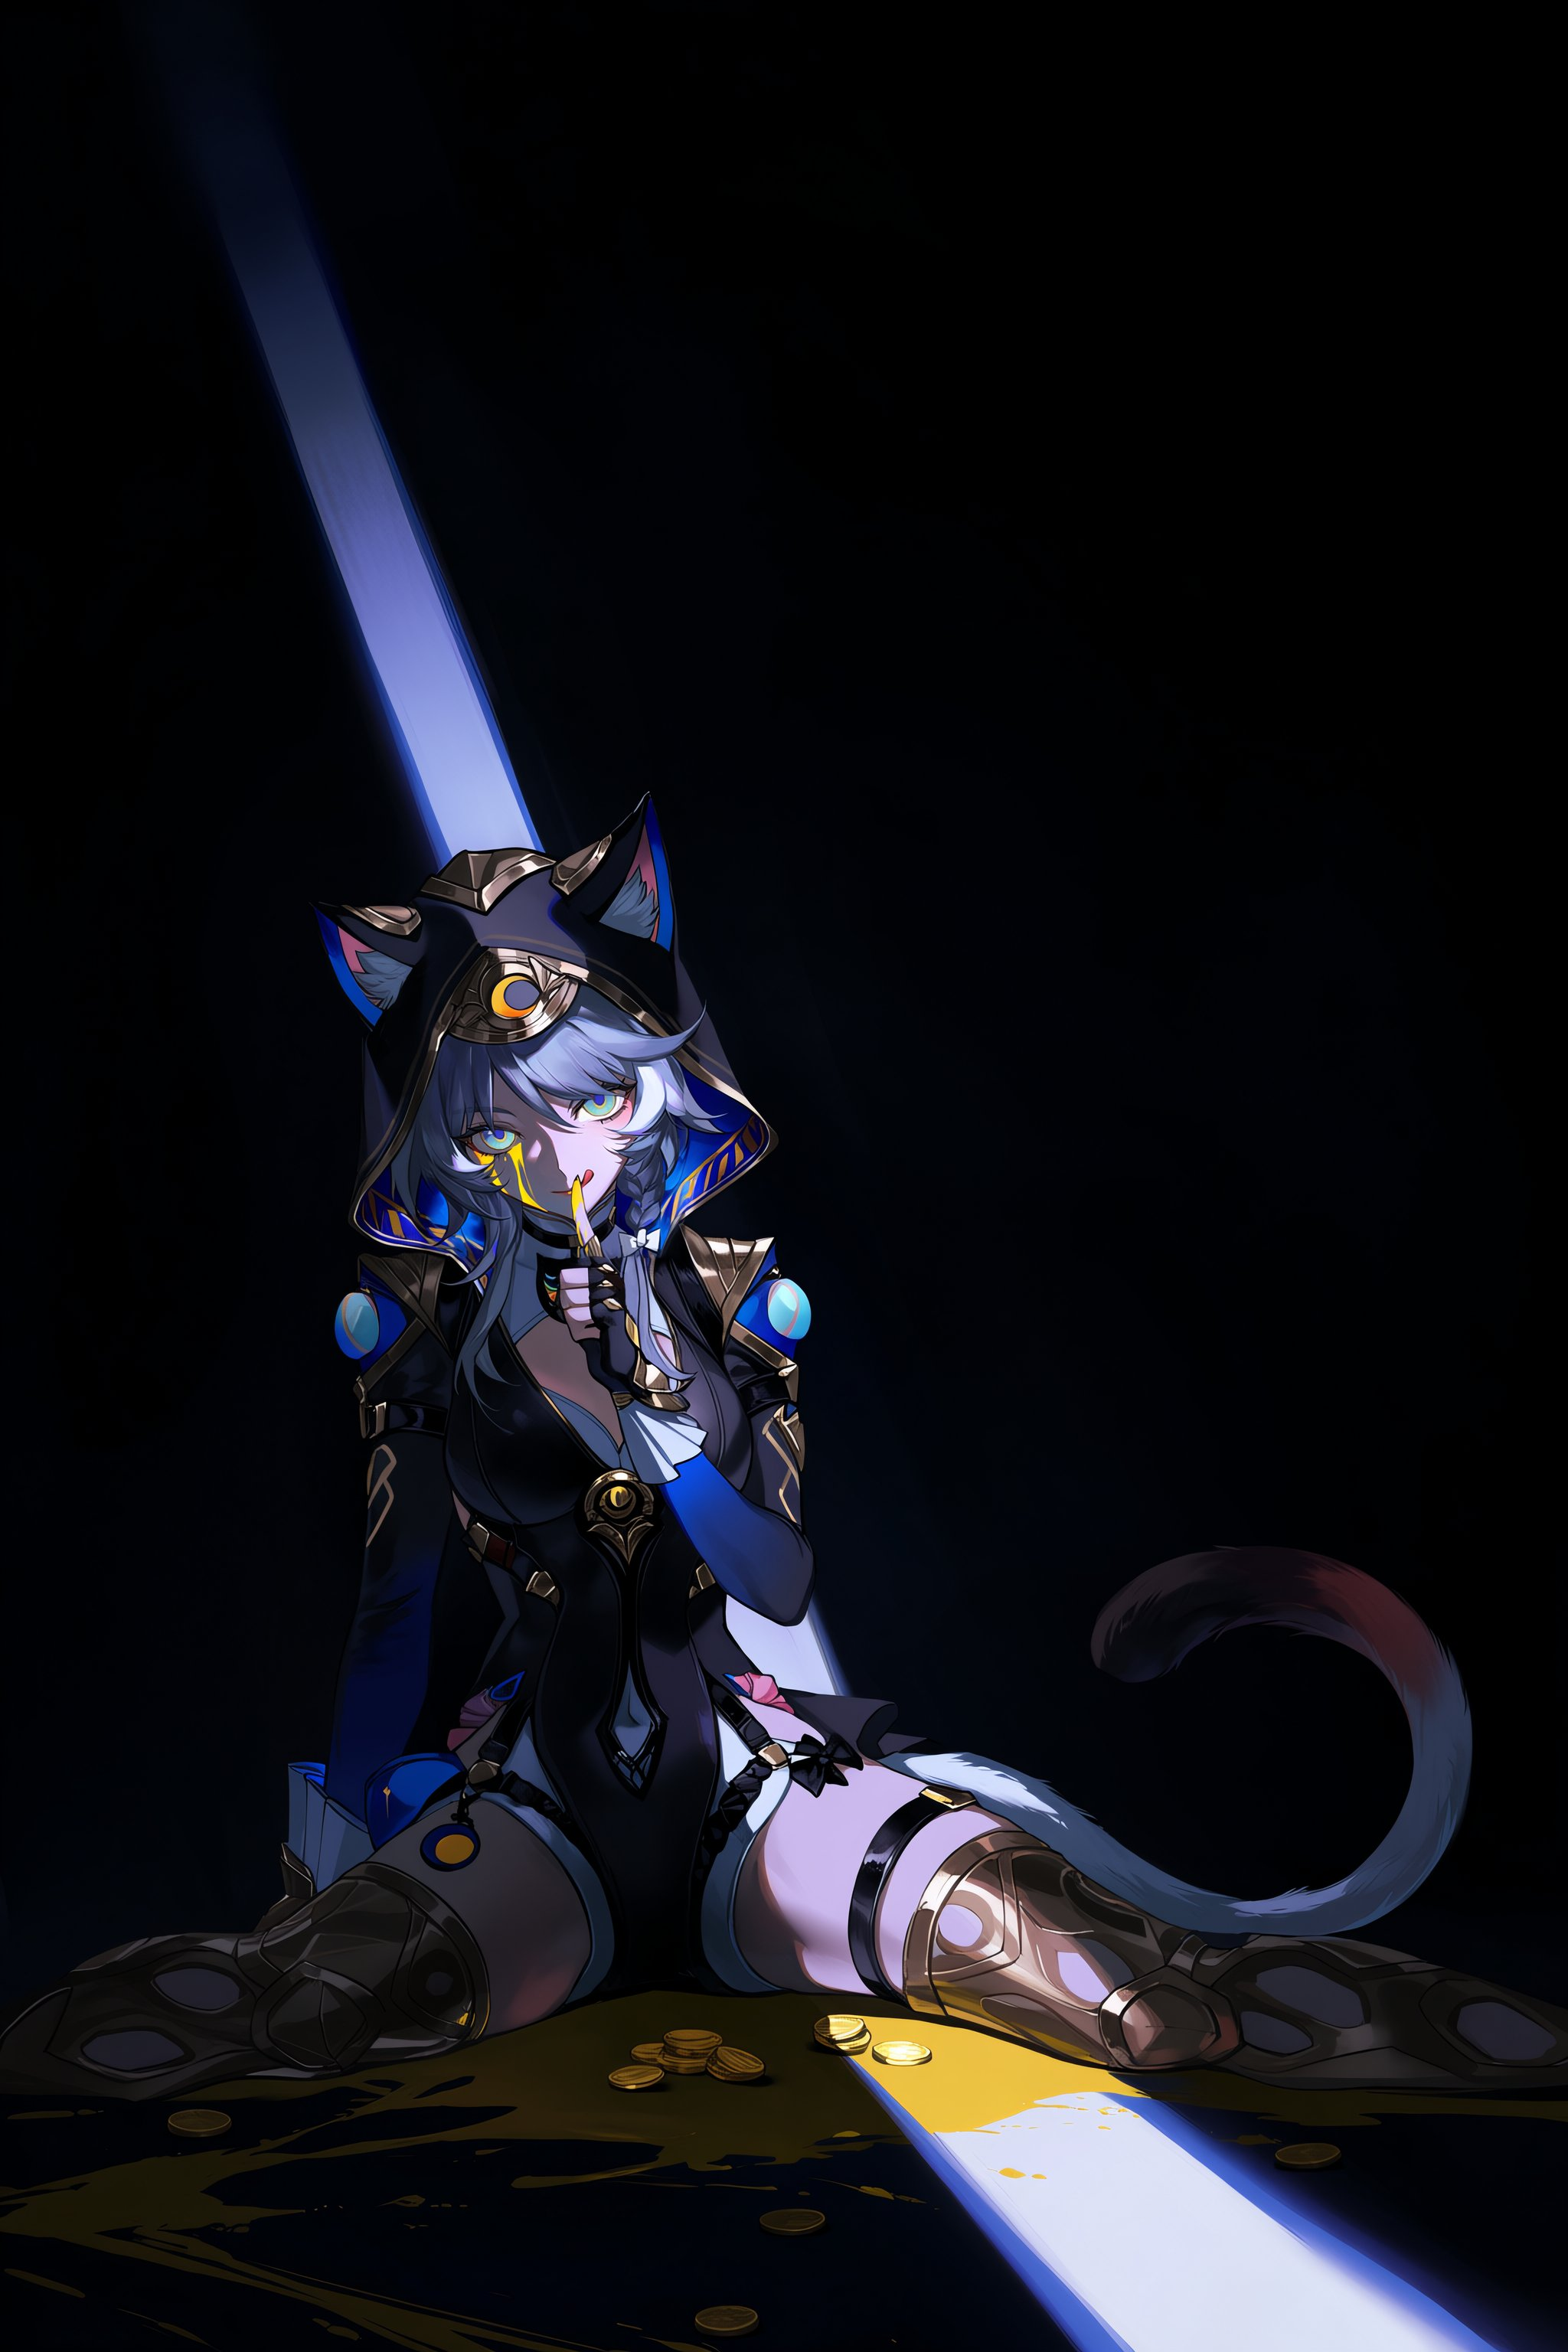
\includegraphics[width=0.632\linewidth]{01705E46-405A-4D35-B256-EFB8333F11DB.JPG}
\end{center}
\newpage
\pagecolor{white}
\color{black}
\tableofcontents
\newpage
\section{Concepts of Computer Science}
\subsection{Computer fundamentals}
\subsubsection{Computer hardware and operation}
\paragraph{Function and interaction of the main CPU components}
The CPU is the critical component that carries out the majority of the processing tasks in a computer system. Consists of:
\begin{itemize}
    \item Control Unit (CU): Directs the operations of the processor. Responsible for the FDE cycle (managing all three operations) + directing the computer's memory, ALU \& I/O devices to carry out the program instructions.
    \item Arithmetic Logic Unit (ALU): Performs arithmetic and logical operations.
    \item Registers: Small, fast storage locations within the CPU that hold data and instructions temporarily during processing.
    \begin{itemize}
        \item Program Counter (PC): Holds the address of the next instruction to be executed.
        \item Memory Address Register (MAR): Holds the address of the memory location that is currently being fetched.
        \item Memory Data Register (MDR): Holds the data that is being transferred to or from memory.
        \item Accumulator (ACC): Holds the result of arithmetic and logical operations performed by the ALU.
        \item Instruction Register (IR): Holds the current instruction being executed.
    \end{itemize}
    \item Buses: Communication pathways that transfer data between the CPU, memory, storage, and I/O devices.
    \begin{itemize}
        \item Data Bus: Transfers data between the CPU, memory, and I/O devices. Bidirectional.
        \item Address Bus: Transfers memory addresses from the CPU to memory. Unidirectional.
        \item Control Bus: Transfers control signals from the CPU to other components. Bidirectional.
    \end{itemize}
\end{itemize}
\textbf{Core:} the processing unit of the CPU. More cores generally means better performance, as multiple cores can handle multiple tasks simultaneously. However, the performance gain depends on the software's ability to utilize multiple cores effectively.\\
Single core processors work well for naturally sequential tasks, while multi-core processors excel in parallel processing tasks.\\
\textbf{Cache:} a small, fast memory located close to the CPU that stores frequently accessed data and instructions. It helps reduce the time it takes for the CPU to access data from main memory. (L1, L2, L3)\\
\textbf{Co-processors:} specialized processors designed to support the main CPU. Tasks from the CPU are offloaded to the co-processor so that they could run in parallel, which can perform them more efficiently. Examples include DSPs, GPUs, and AI accelerators.\\
\textbf{Von Neumann vs Harvard architecture:} Von Neumann architecture uses a single memory space for both instructions and data, while Harvard architecture uses separate memory spaces for instructions and data. Harvard architecture can provide better performance for certain applications, as it allows simultaneous access to both instructions and data. However, it can be more complex to implement and may require more hardware resources.
\paragraph{Role of GPU}
Used to accelerate the rendering of images, videos, and animations. It is particularly effective for tasks that can be parallelized, such as graphics processing and machine learning. 
\begin{itemize}
    \item GPUs have a large number of cores that can handle multiple tasks simultaneously, making them well-suited for tasks that require high computational power.
    \item They also handle the application of shaders and textures to 3D models, which includes lighting, shading and texture mapping. 
    \item GPUs assist in decoding and encoding video streams, which is essential for video playback, video editing, and streaming applications.
    \item Due to the ability to perform parallel processing + matrix and vector operations, GPUs are widely used in machine learning and deep learning applications, where they can accelerate the training and inference of neural networks (esp. for deep learning models).
    \item GPUs also significantly outperformed CPUs in solving cryptographic puzzles, which is why they are widely used in cryptocurrency mining.
\end{itemize} 
\textbf{Accelerators}: separate main circuit board with the processor, memory, power management, etc., but they can not operate by themselves. They are always part of a system (host) in which the CPUs run the operating systems and control the programs execution. (GPU can be one example as well)
\paragraph{Difference between CPU and GPU}
\textbf{Heterogeneous programming}: CPU acts as a main processor, controlling the execution workflow. The host makes all calls, allocates the memory, and handles the memory transfers between CPU and GPU. GPUs run tens of thousands of threads simultaneously on thousands of cores and does not do much of the data management. The device code is executed by doing calls to functions (kernels) written specifically to take advantage of the GPU. \\\\
Overview: The CPU is great for handling various jobs, but the GPU is better for doing the same job many times on a lot of data at once.\\
Usage scenarios:
\begin{itemize}
\item  CPU: Used for general-purpose tasks that require flexibility, quick decisions, and
coordination—such as running an operating system, web browsing, word processing, and managing program instructions.
\item  GPU: Used for tasks involving many similar calculations that can be carried out simultaneously / in parallel, such as rendering graphics in video games, training AI models, machine learning, video editing, and large simulations.
\end{itemize}
\begin{center}
    \begin{tabular}{|p{2.2cm}|p{4.5cm}|p{6.5cm}|p{4.5cm}|}
\hline
\textbf{Processor} & \textbf{Processing} & \textbf{Architecture} & \textbf{Functionality} \\
\hline
CPU & It is a \textbf{general} purpose processor, capable of handling many different tasks. It executes the instructions of computer programs, involving operations such as arithmetic, logic and controlling input / output (I/O) operations, as directed by the operating system. & CPUs generally have fewer cores. Each core is very versatile, making it capable of handling complex computations that require sequential processing. & Allows the user to switch between multiple tasks and applications. This makes it ideal for running the operating system and general software applications. \\
\hline
GPU & It is a \textbf{specialized} processor, with a focus on handling graphics, \textbf{rendering} images, video and animations. & Composed of hundreds or thousands of small cores that are well-suited for tasks that can be run in parallel. While each core is not as powerful as a standard CPU core, the high number of cores allows them to perform a large number of calculations simultaneously, making them perfect for graphical processing. & Suited for tasks that require simultaneous processing of large blocks of data, such as rendering images, video processing and deep learning applications. \\
\hline
\end{tabular}
\end{center}
In case of collaborative efforts to video games operation:
\begin{itemize}
	\item The CPU handles the game’s core logic, including rules, physical calculations and AI behaviour. It processes the inputs from the player.
	\item The GPU renders the game’s visuals. It processes vertex and pixel data to draw images on to the screen, including 3D objects, textures and effects such as lighting and shadows. 
\end{itemize}
\paragraph{Purposes of different types of primary memory}
It directly supports the execution of programs by providing the CPU with fast and flexible access to instructions and data. However, not all primary memory is equal: different types serve distinct purposes, trade-offs, and performance characteristics.
\begin{itemize}
    \item RAM, Random Access Memory: holds instructions and data 
for programs that are currently running. Volatile (loses content when powered off) Directly accessible from CPU. Two types of RAM:
	\begin{itemize}
		\item DRAM: capacitors + transistors (needs to be refreshed)
		\item SRAM: flip flops to store data
	\end{itemize}
    \item ROM, Read-only memory: used for storing instructions that are very rarely modified. (e.g. BIOS: initialize and test the system hardware components on startup, and to load the operating system (OS) software from the secondary memory storage into the RAM) 
    \item Cache (Located within CPU): small, but provides high-speed access to the CPU compared to the RAM. It acts as a buffer between the CPU and the slower RAM, storing frequently used data and instructions. Caches are managed by the cache controller, which uses algorithms like Least Recently Used (LRU) to determine which data to keep or evict.
    \begin{itemize}
        \item L1: located directly on the CPU, making it the fastest type of cache. However, it is also the smallest, often only a few kilobytes in size (32KB to 128KB per core). Each CPU core usually has its own L1 cache:
		\begin{itemize}
			\item L1i to store instructions
			\item L1d to store data
		\end{itemize}
        \item L2: either be on the CPU, or located very near the CPU. L2 cache 
is larger than L1 and can be up to several megabytes in size (256KB to 2MB per core), but slighly slower than L1 cache.
        \item L3: located the furthest from the CPU chip. L3 cache may be shared on multiple-core CPUs. It is the largest of the three, and can be up to tens of megabytes in size (2MB to 64MB shared across all cores). It's also the slowest of all three.
    \end{itemize}
	\item Registers: fastest and smallest type of memory in a computer system. Located directly inside the CPU, they provide temporary storage for data and instructions that the processor is actively using.
\begin{itemize}
\item General-purpose: used to store operands, intermediate results, memory addresses, or anything else the executing program needs.
\item Special-purpose: used by the CPU control unit to manage and coordinate instruction execution. 
\end{itemize}
\end{itemize}
Memory Hierarchy: Register $\Rightarrow$ L1 $\Rightarrow$ L2 $\Rightarrow$ L3 $\Rightarrow$ RAM $\Rightarrow$ Secondary storage.\\\\
\textbf{Cache hit:} data being fetched is located within the cache, reduces retrieval time of data\\
\textbf{Cache miss:} data being fetched is only located within RAM / secondary storage. \\
Types of cache miss:
\begin{itemize}
\item  Compulsory (cold): First-time access to data; it is unavoidable as it is inherent in the first reference to the data.
\item  Capacity: Cache too small to hold all data.
\item  Conflict: Multiple addresses map to the same cache line.
\end{itemize}
The percentage of hit rate determines the efficiency and effectiveness of the cache. Systems with a larger cache size will generally perform better, as well as systems with more intelligent prefetching techniques that can predict which data will be needed soon and load it into cache ahead of time.  
\paragraph{FDE cycle}
\begin{enumerate}
	\item Fetch: The CPU fetches an instruction from the memory. 
	\begin{itemize}
		\item The Program Counter (PC) holds the address of the next instruction to be executed.
		\item This address is copied into the Memory Address Register (MAR).
		\item The address is sent to main memory through the address bus.
		\item The instruction stored at that memory location is sent back to the CPU over the data bus and temporarily held in the Memory Data Register (MDR).
		\item The instruction in the MDR is then transferred to the Current Instruction Register (CIR), where it awaits decoding.
		\item Finally, the PC is incremented so it points to the address of the next instruction.
	\end{itemize}
	\item Decode: The CPU interprets the instruction and prepares the necessary operations to execute it. 
	\begin{itemize}
		\item The CU examines the opcode (the part of the instruction that specifies the operation) and determines what the CPU must do.
\item If the instruction includes operands (addresses or data values), the CU prepares to retrieve them—possibly using the MAR and MDR again for memory access.
\item Internal control signals are generated to direct data movement and select the appropriate ALU operation, register sources, or memory accesses.
	\end{itemize}
	\item Execute: The CPU performs the actions required by the instruction. 
	\begin{itemize}
		\item Arithmetic or logic operations: Data from registers are processed in the ALU, with results stored in the Accumulator (ACC) or another register.
\item Memory operations: The MAR and MDR are used again if data must be read from or written to RAM.
\item Control flow operations: The Program Counter (PC) may be updated.
	\end{itemize}
\end{enumerate}
说老实话，这段IB教科书上写的内容还不如IG时期的教科书，所以我就把去年的拿过来了：
\begin{center}
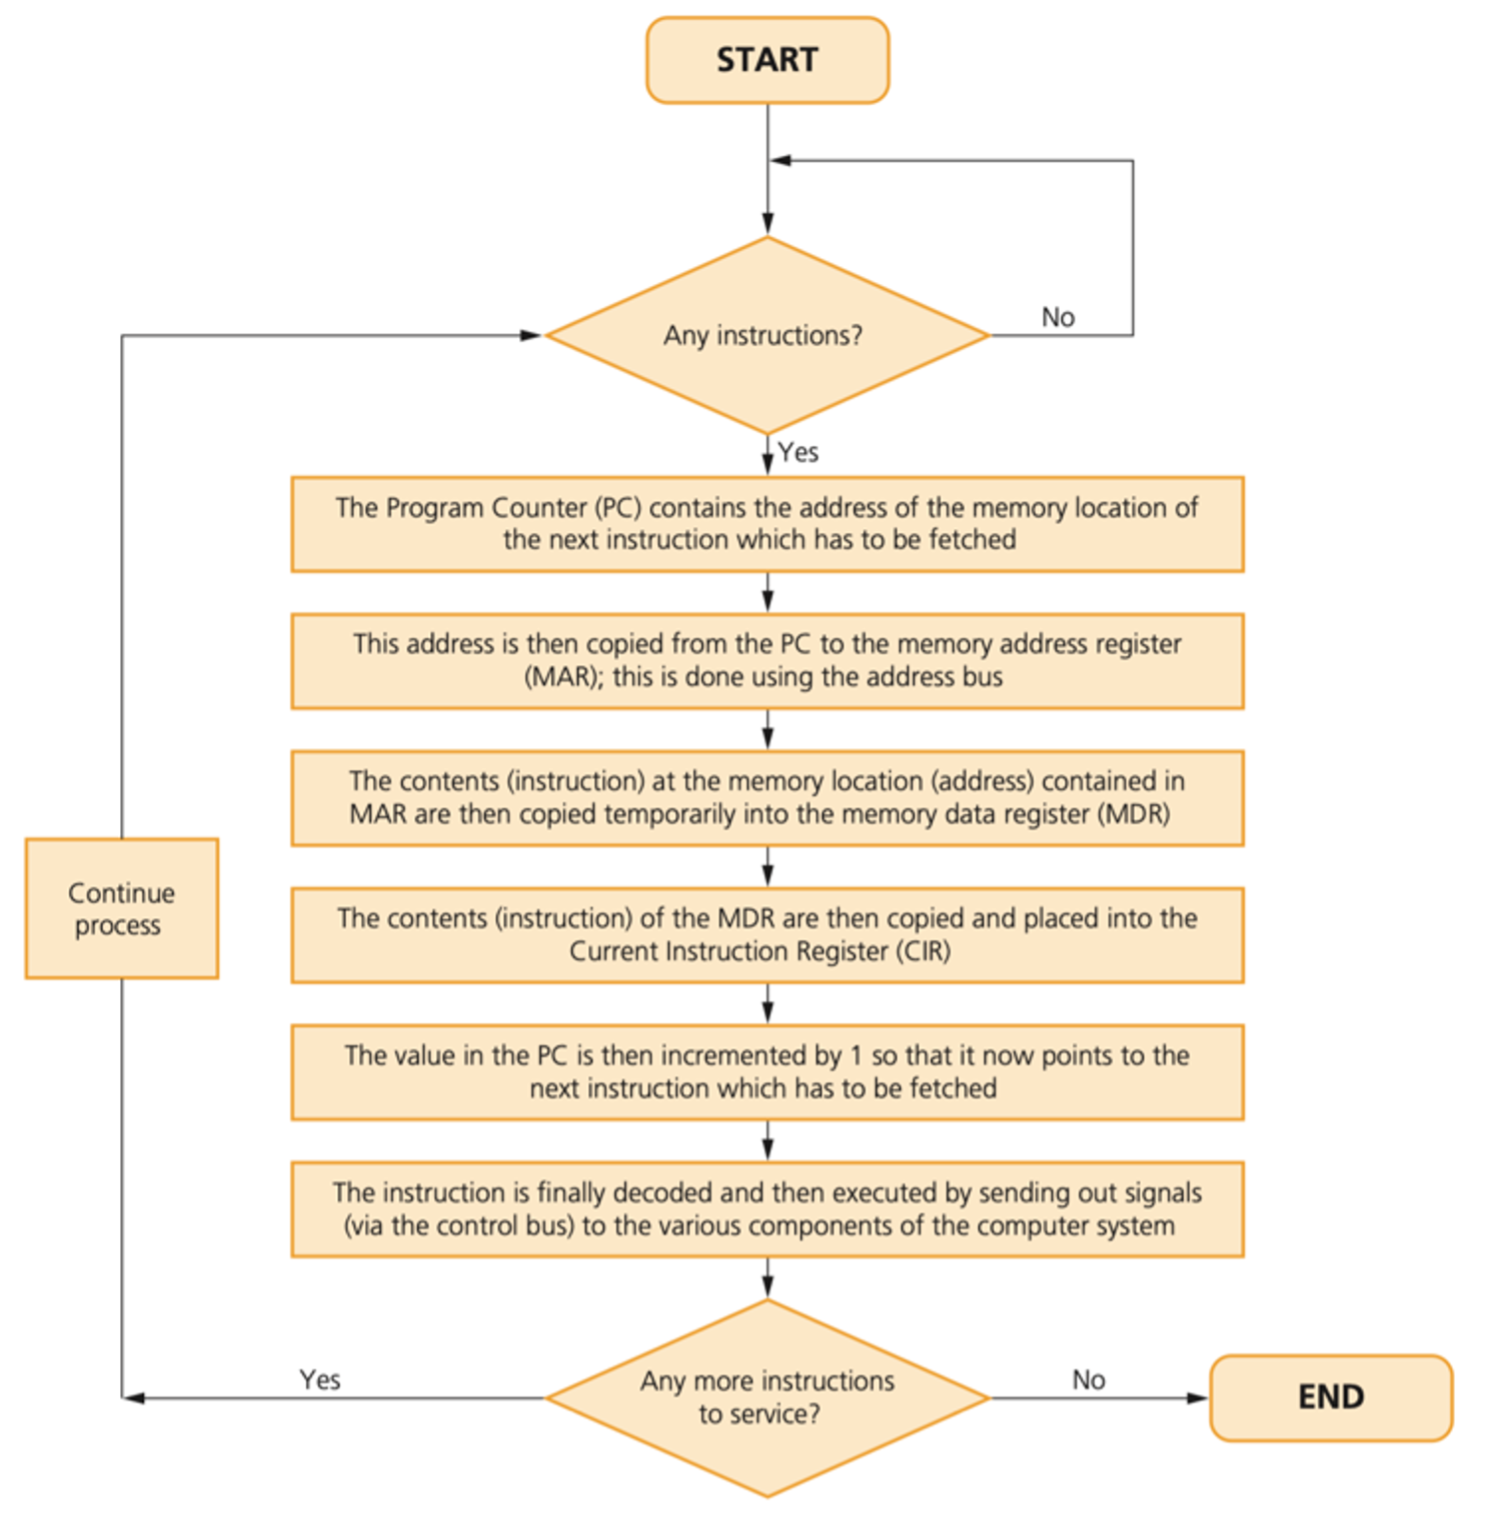
\includegraphics[width=0.9\linewidth]{Picture1.png}
\end{center}
Machine Language: lowest level of programming language that directly corresponds to the instructions executed by a computer's hardware. (In simple terms: binary.)
\paragraph{Pipelining in multi-core architectures}
\paragraph{Internal and external types of secondary memory storage}
\begin{itemize}
	\item Internal Storage
	\begin{itemize}
	\item HDD: utilize a spinning magnetic disk to read / write data. They are suitable for storing large volumes of data, such as media files, backups, and documents, where speed is not so critical. 
	\item SSD: use flash memory to store data, offering high-speed data access and durability. This makes them very popular in portable devices such as laptops and tablets.
	\item eMMC: a type of flash storage that utilizes NAND flash memory. They are soldered directly on to the motherboard of the device. While the capacity and speed do not match a standard SSD, their performance is adequate for basic computing needs and simple applications. 
\end{itemize}
	\item External Storage
\begin{itemize}
\item HDDs \& SSDs: performance and comparison are identical to the internal versions. 
\item Optical discs and optical drives (CD, DVD, blu-rays): cost of an optical disc is low compared to an HDD or SSD and, while their read / write speeds may be slower, they are sufficient for data archiving and playback. However, the discs are prone to scratches, especially if they are not stored correctly, and they require an optical drive to read and write to them.
\item Memory cards (SD, microSD, CF): compact storage devices often used in cameras, smartphones and other portable devices. They are ideal for expanding storage in mobile devices and for storing photos 
and videos in cameras, using NAND flash memory. Highly durable; read / write times are generally slower 
than SSDs, but outperform those of optical discs. 
\item NAS: dedicated file storage connected to a network that allows multiple users to access 
data. It is often used in homes or businesses for centralizing data storage, file storage 
and data backup. Usually made up of multiple HDDs and SSDs configured in RAIDs. It is normally connected to the network via Ethernet, and runs a lightweight operating system designed for file storage, and the management and sharing of files. 
\end{itemize}
\end{itemize}
Comparison between HDDs and SSDs:
\begin{center}
\begin{tabular}{|p{4cm}|p{6.5cm}|p{6.5cm}|}
        \hline
        \textbf{Feature} & \textbf{HDD (hard disk drive)} & \textbf{SSD (solid state drive)} \\
        \hline
        Storage technology & Magnetic storage with spinning disks and read / write heads & Flash memory with no moving parts \\
        \hline
        Speed & Slower read / write speeds (generally 50--150 MB/s) & Faster read / write speeds (generally 200--500 MB/s) \\
        \hline
        Durability & More prone to physical damage due to moving parts & More durable; resistant to physical shock \\
        \hline
        Noise & Produces noise due to moving parts & Silent operation \\
        \hline
        Power consumption & Higher power usage due to mechanical parts & Lower power consumption \\
        \hline
        Cost & Generally cheaper per GB & More expensive per GB \\
        \hline
        Capacity & Available in larger capacities (up to several TB) & Typically available in smaller capacities (up to several TB, but at a higher cost) \\
        \hline
        Weight & Heavier due to mechanical components & Lighter \\
        \hline
        Heat generation & Generates more heat due to moving parts & Generates less heat \\
        \hline
    \end{tabular}
\end{center}

\paragraph{Compression}
\begin{itemize}
\item Lossy: reduces files by permanently eliminating certain information. This information 
is redundant or less critical data, resulting in a compressed version that is not identical 
to the original but is, ideally, indistinguishable from the original to human senses.
\begin{itemize}
\item Transform encoding: 
\begin{center}
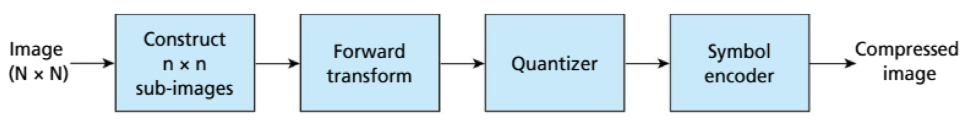
\includegraphics[width=0.8\linewidth]{Screenshot 2026-09-17 at 23.00.02.png}
\end{center}
\begin{enumerate}
\item Transform coding takes an image of N $\times$ N size and sections it into smaller sub-images of size n $\times$ n. 
\item Then the forward transform is carried out on each of the sub-images. The forward transform can use different algorithms, depending on the type of file compression, but for JPEGs DCT (discrete cosine transform) is used. This takes the image data from the spatial domain (pixel values) to the frequency domain. The output breaks the sub-image down into low- and high-frequency coefficients.
\begin{itemize}
\item Low-frequency data: correspond to slow changes in pixel values, such as broad areas. 
\item High-frequency data: correspond to rapid changes in pixel values, representing fine details, edges and textures. 
\end{itemize} 
\item These frequency coetficients are then passed to the quantizer. This step significantly reduces file size by simplifying the frequency coefficients obtained from the DCT. The purpose of quantization is to reduce the precision of high-frequency components (the fine details) rather than low-frequency components. This is because the human eye is less sensitive to high-frequency data loss compared to low-frequency detail. The extent of the quantization decides the compression level and the quality of the final image.
\item The final step of transform coding is the symbol encoder. This is where the quantized coefficients are further compressed using entropy coding techniques. This runs through three further algorithms to reduce the file size by efficiently representing the frequency of occurrence of each symbol. The algorithms used at this stage are 
\begin{enumerate}
\item Zigzag scan
\item RLE
\item Huffman coding
\end{enumerate}
\end{enumerate}
\end{itemize}
\item Lossless: data is compressed to a smaller size, but can be restored back to the original without any loss of information. This technique works by identifying and eliminating statistical redundancy within the data, and this process can be reversed when needed. 
	\begin{itemize}
		\item Run-length encoding: used to reduce the
size of files containing many consecutive repeated characters. The original string of info is represented by the recurrence of the letter + the letter itself. RLE is straightforward to implement and it is very effective for data with lots of repetitions, such as simple graphics and certain types of text file
	\end{itemize}
\end{itemize}
\paragraph{Type of services in cloud implementation}
\begin{itemize}
\item SaaS: delivers software applications over the internet. SaaS provides a cost-effective and convenient solution for businesses and individuals, offering a wide range of applications from productivity tools to customer-relationship management systems. 
\item PaaS: provides a cloud-based platform that allows developers to build, test and deploy applications without managing the underlying infrastructure. PaaS includes tools \& services to facilitate application development, such as databases, middleware (software that connects different applications) and dev frameworks. PaaS accelerates software development by allowing developers to focus on coding rather than infrastructure management.
\item IaaS: provides virtualized computing resources over the internet, such as virtual machines, storage and networks. IaaS gives users full control over their virtual machines and networks. This reduces the need for upfront investment in hardware and allows businesses to rent solutions at a lower initial cost using a subscription model. IaaS is also scalable, making it easy to adjust resources as the user base grows.
\end{itemize}
\subsubsection{Data representation and computer logic}
都是老生常谈的东西，看看就好。金波尔万岁！！！
\paragraph{Principal methods of representing data}
Modern computing ultimately settled on binary (base-2) as the primary number system. The base-2 system represents two possible states: 1 or 0. The binary system is particularly well-suited to represent the state of electrical switches within a computer system: on (1) and off (0). This simplicity reduces hardware complexity and enhances reliability. \\\\
The increased reliability of binary systems stems from their use of only two states. Small 
variations in signal strength do not affect data integrity as much as in systems using larger bases, making binary more robust in noisy (electrical disturbances) environments. 
\[
\begin{array}{|c|c|}
\hline
\textbf{Conversion} & \textbf{Method} \\ \hline

\text{Binary} \rightarrow \text{Decimal}
&
\begin{array}{l}
\text{Multiply each binary digit by its corresponding power of }2,\\
\text{then add the results.}\\
1011_2 = 1(2^3)+0(2^2)+1(2^1)+1(2^0)\\
\phantom{1011_2}=8+0+2+1=11_{10}
\end{array}
\\ \hline

\text{Decimal} \rightarrow \text{Binary}
&
\begin{array}{l}
\text{Repeatedly divide the decimal number by }2,\\
\text{record the remainders, and read them from bottom to top.}\\
\text{I'd personally recommend the subtraction method.}\\
\text{(Subtract the decimal number by powers of 2 and record the results.)}\\
\text{If you use this method, remember to start with the most significant bit (MSB)}\\\text{the left most bit, not the least significant bit (LSB) (which is the right most bit.) }
\end{array}
\\ \hline

\end{array}
\]
Base-2 vs Base-10:
\begin{center}
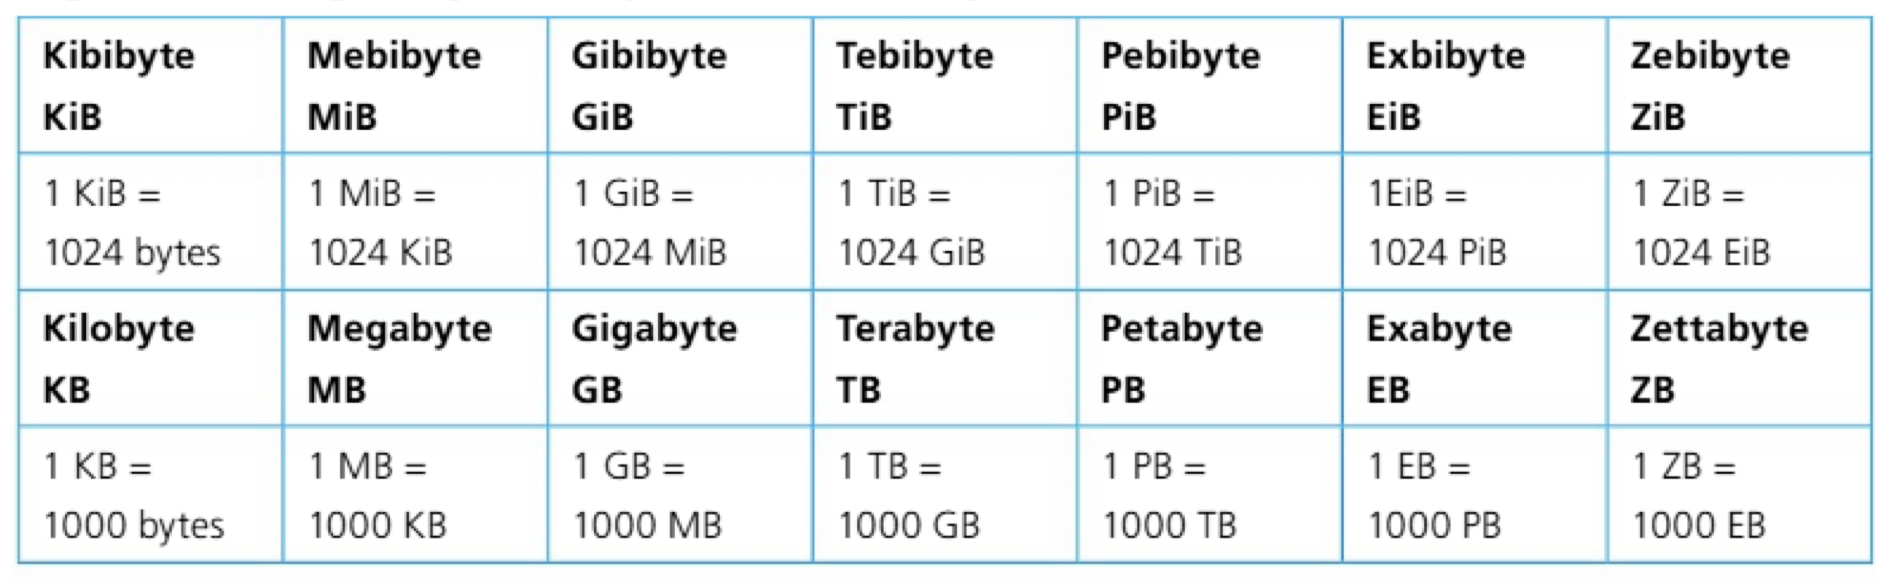
\includegraphics[width=0.9\linewidth]{Screenshot 2026-09-24 at 12.41.11.png}
\end{center}
1 byte = 8 bits, 1 nibble = 4 bits. Note here that KB and Kb are different units. ($KB=8\times Kb$)\\\\
Hexadecimal: base-16 number system, where 10 - 15 are represented by A to F.\\
Reasons for using hexadecimal: 
\begin{itemize}
    \item Ease of conversion between binary and hexadecimal
    \item Compact size of display (used in debugging tools, memory dumps and assembly language programming)
\end{itemize}
Conversion of hexadecimal $\Leftrightarrow$ binary: split the binary in nibbles and turn into hexadecimal for assembling the result. The reverse also stands; i.e. convert each hexadecimal character to binary nibbles, and assemble them in the correct order. (For decimal conversion, I recommend conversion to binary first and then convert to hexadecimal) 
\paragraph{How binary is used to store data}
\begin{itemize}
    \item Characters and strings
    \begin{itemize}
        \item ASCII encoding: designed to provide a common standard for the interchange of text data. Initially started out as 7-bit encoding system (later 8 bits for more character support). Taking the 8-bit system as an example:
\begin{itemize}
    \item $010.....$ represents uppercase letters, while $011.....$ represents lowercase letters.
    \item The last 5 digits, when converted from binary to decimal, corresponds to the alphabet letters (e.g. 1 $\rightarrow$ a, 2 $\rightarrow$ b)
\end{itemize}
	\item Unicode encoding: provides a unique number for every character, regardless of platform, program or language. Few different versions of Unicode:
	\begin{center}
		\renewcommand{\arraystretch}{1.5}
\begin{tabular}{|p{2cm}|p{4cm}|p{5.5cm}|p{4cm}|}
\hline
& \textbf{UTF-8} & \textbf{UTF-16} & \textbf{UTF-32} \\
\hline
\textbf{Variable length encoding} & 1--4 bytes per character & 2 or 4 bytes per character & 4 bytes per character \\
\hline
\textbf{Note} & Compatibility: backward compatible with ASCII & Surrogate pairs: for characters outside the \textbf{Basic Multilingual Plane} (the 
maost commonly used characters and symbals for almost all modern 
languages), two 16-bit code units are used & Simplicity: easier to process because each character is exactly 4 bytes \\
\hline
\textbf{Usage} & Most commonly used encoding on the web and in many applications & Often used in Windows and Java environments & Less common due to higher storage requirements \\
\hline
\end{tabular}
	\end{center}
\item Using UTF-8 as an example: (essentially kept ASCII but added some other bytes in a clever way): 11110000 10011111 10011000 10000100
\begin{itemize}
   \item $11110000$: 1111 means 4 bytes is needed to transmit the character, the 0 coming right after the 4 1s means the end of transmitting the number of bytes. The 3 0s afterwards are the data transmitted.
   \item $10......$: 10 means the continuation bytes being sent, the numbers afterwards are transmitted data.
   \item 0001 1111 0110 0000 0100 are the final data received.
   \end{itemize}
\item UTF-8 has been adopted by the internet as the main character encoding system. Some problems:
\begin{itemize}
    \item Due to the variable length, some characterstake more space compared to single-byte encodings. 
    \item ... This can lead to larger file sizes in certain contexts.
    \item The processing required to handle variable length encoding also requires more complex \\ processing compared to fixed-length 
systems such as UTF-32. 
    \end{itemize}
    \end{itemize}
    \item Images
    \begin{itemize}
        \item Bitmap / raster images: reproduce images by using a grid of pixels, with each pixel assigned a specific colour and intensity. Some key concepts:
        \begin{itemize}
            \item Pixel: short for "picture element", the smallest unit of a digital image / display, representing a single point in the image with a specific color and intensity.
            \item Image resolution: the number of pixels contained within a digital image, typically expressed as the dimensions (width $\times$ height) in pixels, and sometimes as the pixel density (PPI/ DPI) for print quality. 
            \item Color / bit depth: the amount of bits used to describe the color
            \item Formula for calculating image size:
            \[\text{image size (bits) = width}\times \text{height} \times \text{bit depth}\]
However, in reality, this calculation is not completely accurate, as the image would require 
more data to store metadata and other header information.
            \item Metadata: information that describes other data, providing context and details about the data's content, structure and attributes.
        \end{itemize}
		\item Ways to improve the image quality:
		\begin{itemize}
		    \item Increase image resolution. A higher resolution allows for greater detail and clarity. The trade-off for a higher resolution image is larger file size, which can impact storage and transfer efficiency. 依旧老生常谈
		    \item Increase color depth. When we increase the colour depth, it allows for a wider range of colours to be represented, resulting in more vibrant and accurate images. $2^\text{bit depth}=$ numbers of color available for representation. Mostly 24 bits for modern photos.
		\end{itemize}
	\item When working with graphics, RGB values are often shown in hexadecimal. 
    \end{itemize}
    \item Audio: (analog) a continuous signal that represents sound waves through variations of air pressure. These sound waves can be captured through input devices, such as microphones, which convert the sound waves into a digital signal, which is stored as binary. Process: (金波儿老生常谈）
    \begin{enumerate}
        \item An analog to digital converter(ADC) samples the amplitude (loudness) of the sound at discrete intervals in a process known as sampling. The rate at which this happens is measured in Hertz (Hz) — the higher the Hertz, the more samples are recorded per second.
        \begin{itemize}
            \item Amplitude: the magnitude of change in a sound wave, representing the loudness or intensity of the sound. 
            \item  Sampling: the process of converting a continuous analogue signal into a series of discrete digital values by measuring the signal’s amplitude at regular intervals. 
        \end{itemize}
		\item This sample 1s then stored and represented as a numerical value in binary. The precision is determined by the bit depth. The larger the bit depth, the more possible values that can be used to describe the sample.
		\item Formula for calculating audio size:
		\[\text{file size (bits)}=\text{sampling rate}\times \text{bit depth}\times\text{\# of channels}\]
		\item Many formats to choose from for storing audio files: (They mainly differ by whether they are compressed or uncompressed)
		\begin{itemize}
		    \item Uncompressed formats store the raw binary data (e.g. WAV, AIFF)
		    \item Compressed formats use algorithms to reduce the file size for storage or transmission (e.g. MP3, FLAC)
		    \end{itemize}
        \end{enumerate}
    \item Video
    \begin{itemize}
        \item Components include:
        \begin{itemize}
            \item Frames (visual)
            \begin{itemize}
                \item In their raw form, frames are stored the same as images, with each pixel having a value that can be represented using a colour model such as RGB.
                \item To improve colour efficiency, frames are often converted from the RGB colour model to a different one such as YUV. This helps with compression, as this colour model emphasizes luminance (brightness), which the human eye is more sensitive to than changes in colour detail. 
                \end{itemize}
            \item Audio tracks
            \item Metadata
            \item Subtitles and closed captions
            \end{itemize}
			\item Compression methods / techniques
			\begin{itemize}
			    \item Spatial compression: particularly effective and commonly used for video that has significant detail variation in each frame. It reduces file size by eliminating redundant information within each frame, such as colour depth or detail levels.
			    \item Temporal compression: particularly effective and commonly used for video that has consistent motion across frames. It reduces file size by eliminating redundant information between consecutive frames, capturing only the changes or movements from one frame to the next. As a predictive compression technique, it predicts frame content based on the preceding and sometimes following frames, only storing the differences.
			    \end{itemize}
        \end{itemize}
\end{itemize}
Different binary methods for storing integers:
\begin{itemize}
    \item Unsigned binary (covered in A1.2.1)
    \item Signed binary (negative + positive):
    \begin{itemize}
        \item Two's complement: most significant bit represents sign. 0 for positive, 1 for negative. To convert a positive binary number to its negative counterpart in two’s complement, you first invert all the bits and then add 1 to the least significant bit.
        \item One’s complement: To obtain the one’s complement of a positive number, you simply invert all the bits (change 0s to 1s and 1s to 0s). One's complement have TWO (positive and negative) zeros.
        \item Sign-magnitude: most significant bit serves for sign; the remaining bits represent the magnitude of the number, like how unsigned binary numbers work. 
        \end{itemize}
\item Binary-coded decimal: method of representing decimal numbers where each digit of the decimal number is encoded separately into its own binary form. BCD assigns a 4-bit binary code to each decimal digit (0-9). 
\item Gray code (reflected binary code): a binary system where two successive values are only allowed to differ by one bit.
\begin{center}
\begin{tabular}{|c|c|c|}
\hline
\textbf{Decimal} & \textbf{3-bit binary} & \textbf{3-bit Gray code} \\
\hline
0 & 000 & 000 \\
1 & 001 & 001 \\
2 & 010 & 011 \\
3 & 011 & 010 \\
4 & 100 & 110 \\
5 & 101 & 111 \\
6 & 110 & 101 \\
7 & 111 & 100 \\
\hline
\end{tabular}
\end{center}
For example, from decimal 3 to 4, ordinary binary changes from 011 to 100 (three bits change), while Gray code changes from 010 to 110 (only one bit changes).
\item Excess-N (biased representation): a fixed bias (N) is added to the actual value to form an encoded value, and you subtract this bias to decode it. This is used to make all signed integers appear as non-negative binary numbers to allow for easier comparisons and arithmetic operations. 我打算法题的时候有一次这么干过XD
\item Fixed-point representation: a method used to store real numbers (numbers with fractional parts) in binary by fixing the position of the binary point. In a fixed-point system, the binary point is placed at a predetermined position, either between certain bits or at a specific location in the binary sequence. This allows for a straightforward representation of fractional numbers, though with some trade-offs in terms of precision and range.
\item Floating-point representation: a method used to represent real numbers that can have a very large range or fractional parts. It does this by storing numbers in a format that includes a sign, an exponent and a mantissa (or significand).
\begin{enumerate}
    \item Sign bit (one bit): The sign bit determines whether the number is positive or negative. 
    \item Exponent (eight bits): 
This is used to scale the number by a power of two and is stored using the Excess-127 system in its “biased” form.
\item Mantissa (23 bits): 
This represents the significant digits of the number. The mantissa does not store leading ones (in normalized form, $1.xxxxxx\times 2^n$). 
\end{enumerate}
An example of FP representation (32-bit single precision): represent $13.25_{10}$.
\begin{enumerate}
    \item Convert to binary and normalize:
    \[
    13.25_{10} = 1101.01_2 = 1.10101_2 \times 2^3.
    \]
    \item Sign bit: the number is positive, so the sign bit is \texttt{0}.
    \item Exponent: add the bias of 127 to the actual exponent, giving $3 + 127 = 130_{10} = 10000010_2$.
    \item Mantissa: omit the implicit leading 1 and store the fractional bits \texttt{10101}, padded with zeros to 23 bits: \texttt{10101000000000000000000}.
\end{enumerate}
The stored representation is:
\[
\underbrace{\texttt{0}}_{\text{Sign (1 bit)}}\;\vert\;
\underbrace{\texttt{10000010}}_{\text{Exponent (8 bits)}}\;\vert\;
\underbrace{\texttt{10101000000000000000000}}_{\text{Mantissa (23 bits)}}.
\]
To decode it, subtract the exponent bias and restore the implicit leading 1:
\[
(-1)^0 \times (1 + 2^{-1} + 2^{-3} + 2^{-5}) \times 2^{130-127}
= 1.65625 \times 8 = 13.25.
\]
\end{itemize}
\paragraph{Purpose and use of logic gates}
Logic gates are made up of transistors, which act as electronic switches, allowing or blocking the flow of electrical current. In a transistor, the control wire (or “gate”) regulates the current between the two electrodes, known as the “source” and the “drain”. When voltage is applied to the gate, it allows current to flow from the source to the drain, enabling the transistor to switch states and perform logical operations.
\begin{center}

\renewcommand{\arraystretch}{1.15}
\setlength{\tabcolsep}{8pt}

% =========================
% AND
% =========================
\begin{minipage}{0.22\textwidth}
\centering
\begin{circuitikz}
    \node[and port] (G) {};
    \draw (G.in 1) -- ++(-0.6,0);
    \draw (G.in 2) -- ++(-0.6,0);
    \draw (G.out) -- ++(0.6,0);
\end{circuitikz}
\vspace{3mm}

\textbf{AND}

$Y = A \cdot B$

\[
\begin{array}{cc|c}
A & B & Y \\ \hline
0 & 0 & 0 \\
0 & 1 & 0 \\
1 & 0 & 0 \\
1 & 1 & 1
\end{array}
\]

\vspace{2mm}

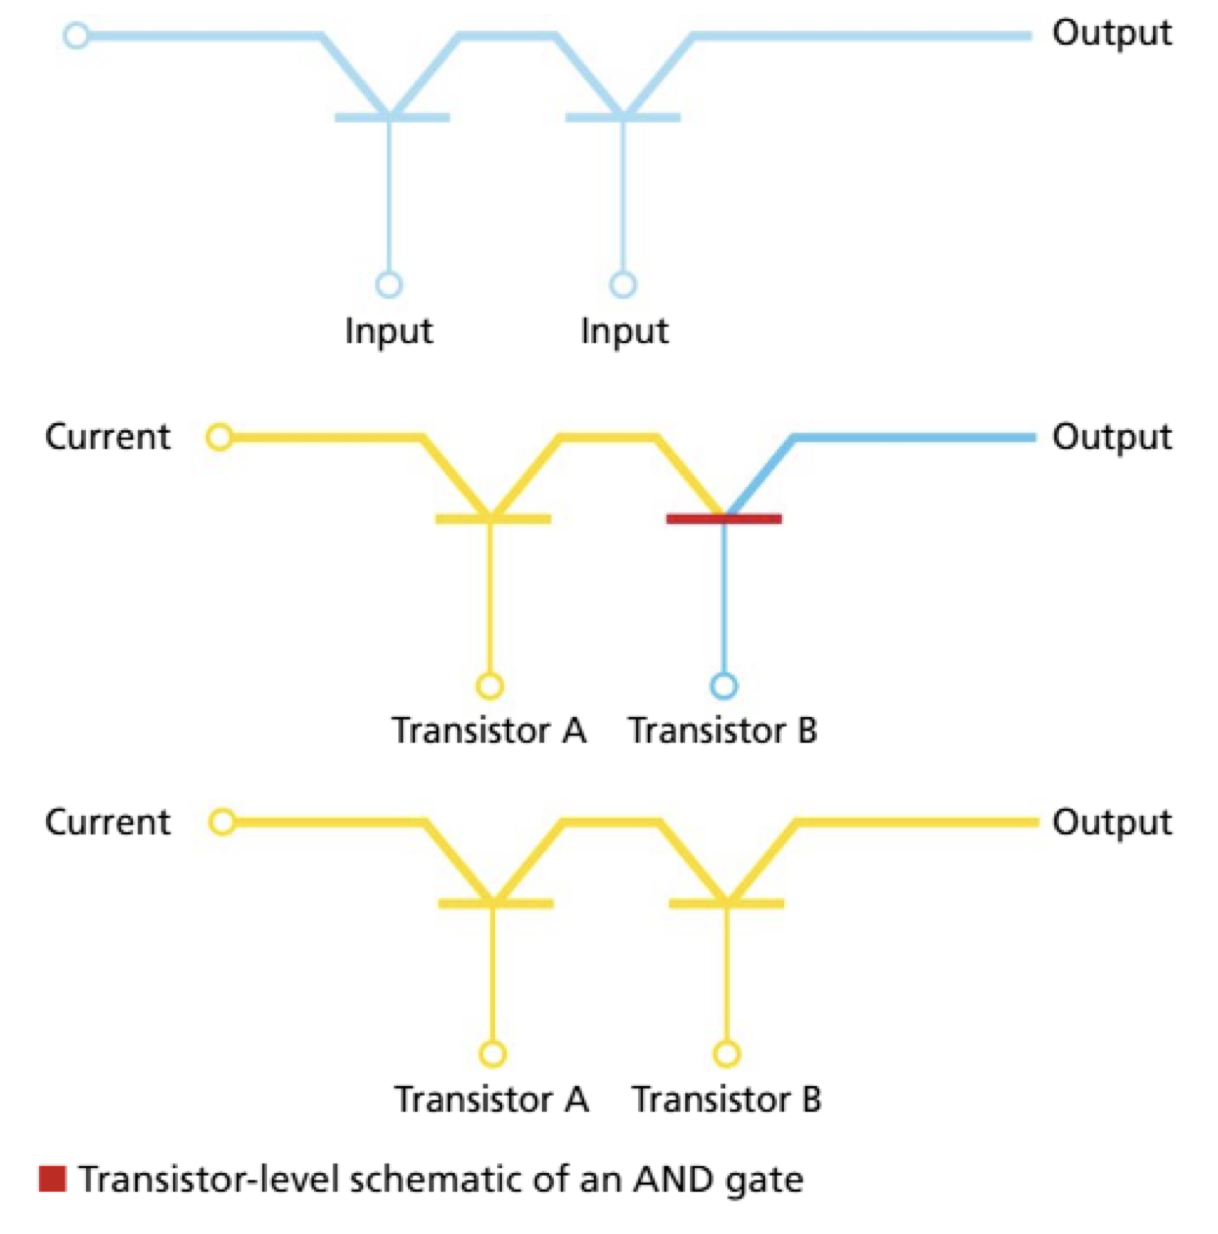
\includegraphics[width=\linewidth]{Screenshot 2026-10-05 at 12.33.38.png}

\end{minipage}
\hfill
% =========================
% OR
% =========================
\begin{minipage}{0.22\textwidth}
\centering
\begin{circuitikz}
    \node[or port] (G) {};
    \draw (G.in 1) -- ++(-0.6,0);
    \draw (G.in 2) -- ++(-0.6,0);
    \draw (G.out) -- ++(0.6,0);
\end{circuitikz}

\vspace{3mm}

\textbf{OR}

$Y = A + B$

\[
\begin{array}{cc|c}
A & B & Y \\ \hline
0 & 0 & 0 \\
0 & 1 & 1 \\
1 & 0 & 1 \\
1 & 1 & 1
\end{array}
\]

\vspace{2mm}

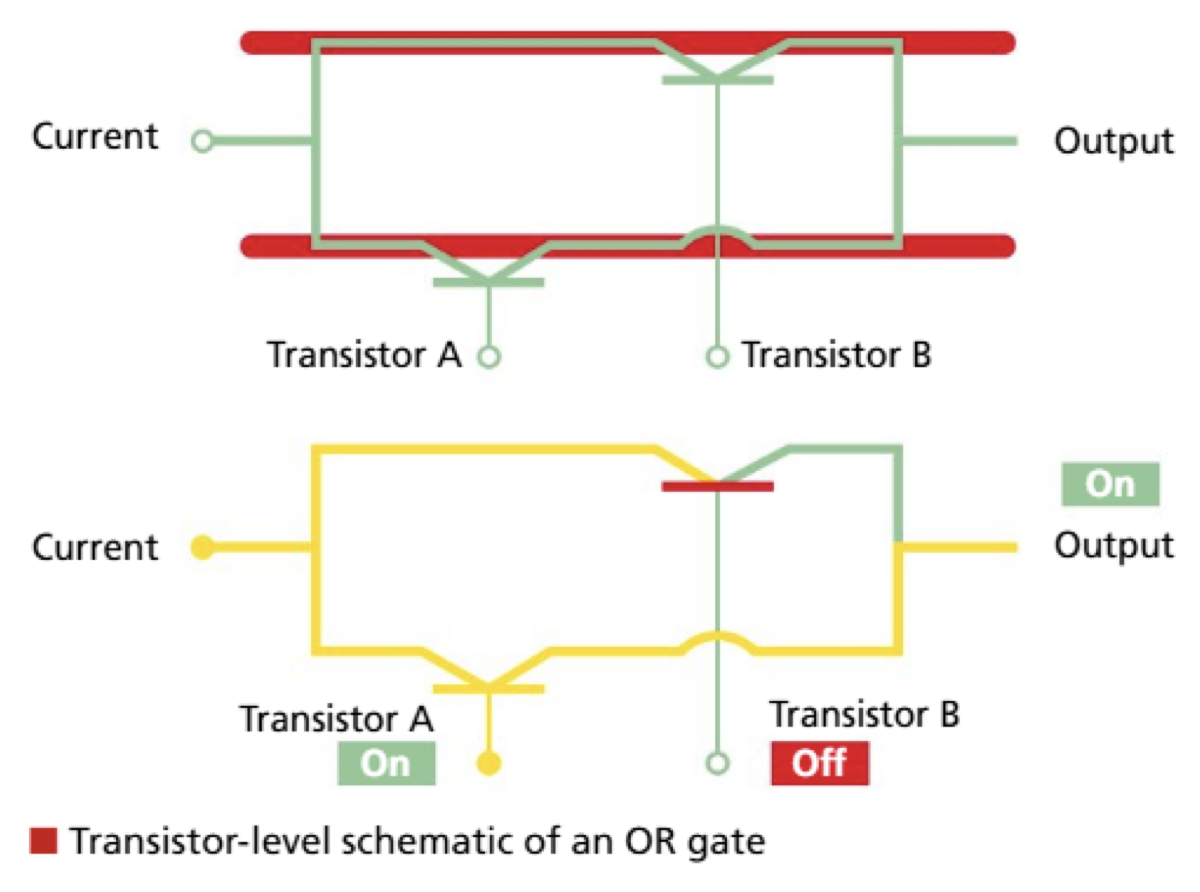
\includegraphics[width=\linewidth]{Screenshot 2026-10-05 at 12.34.03.png}

\end{minipage}
\hfill
% =========================
% NOT
% =========================
\begin{minipage}{0.22\textwidth}
\centering
\begin{circuitikz}
    \node[not port] (G) {};
    \draw (G.in) -- ++(-0.6,0);
    \draw (G.out) -- ++(0.6,0);
\end{circuitikz}

\vspace{3mm}

\textbf{NOT}

$Y = \overline{A}$

\[
\begin{array}{c|c}
A & Y \\ \hline
0 & 1 \\
1 & 0
\end{array}
\]

\vspace{2mm}

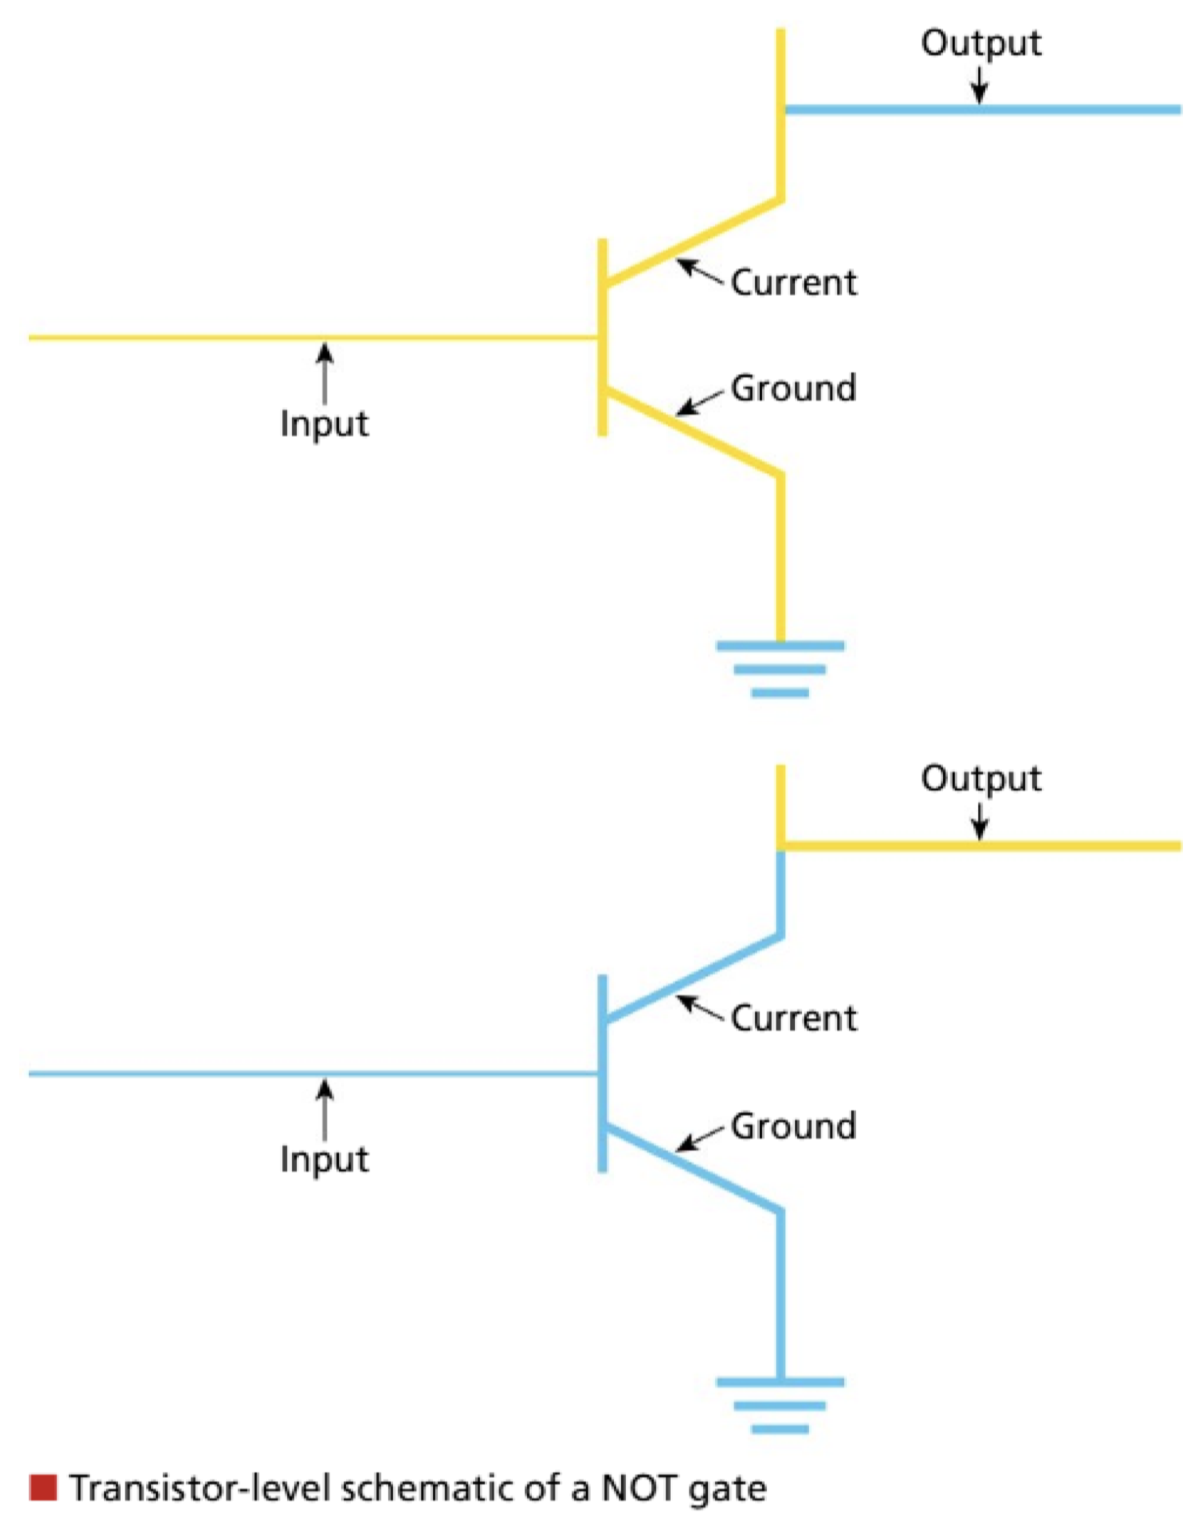
\includegraphics[width=\linewidth]{Screenshot 2026-10-05 at 12.37.18.png}

\end{minipage}
\hfill
% =========================
% BUFFER
% =========================
\begin{minipage}{0.22\textwidth}
\centering
\begin{circuitikz}
    \node[buffer port] (G) {};
    \draw (G.in) -- ++(-0.6,0);
    \draw (G.out) -- ++(0.6,0);
\end{circuitikz}

\vspace{3mm}

\textbf{BUFFER}

$Y = A$

\[
\begin{array}{c|c}
A & Y \\ \hline
0 & 0 \\
1 & 1
\end{array}
\]

\vspace{2mm}

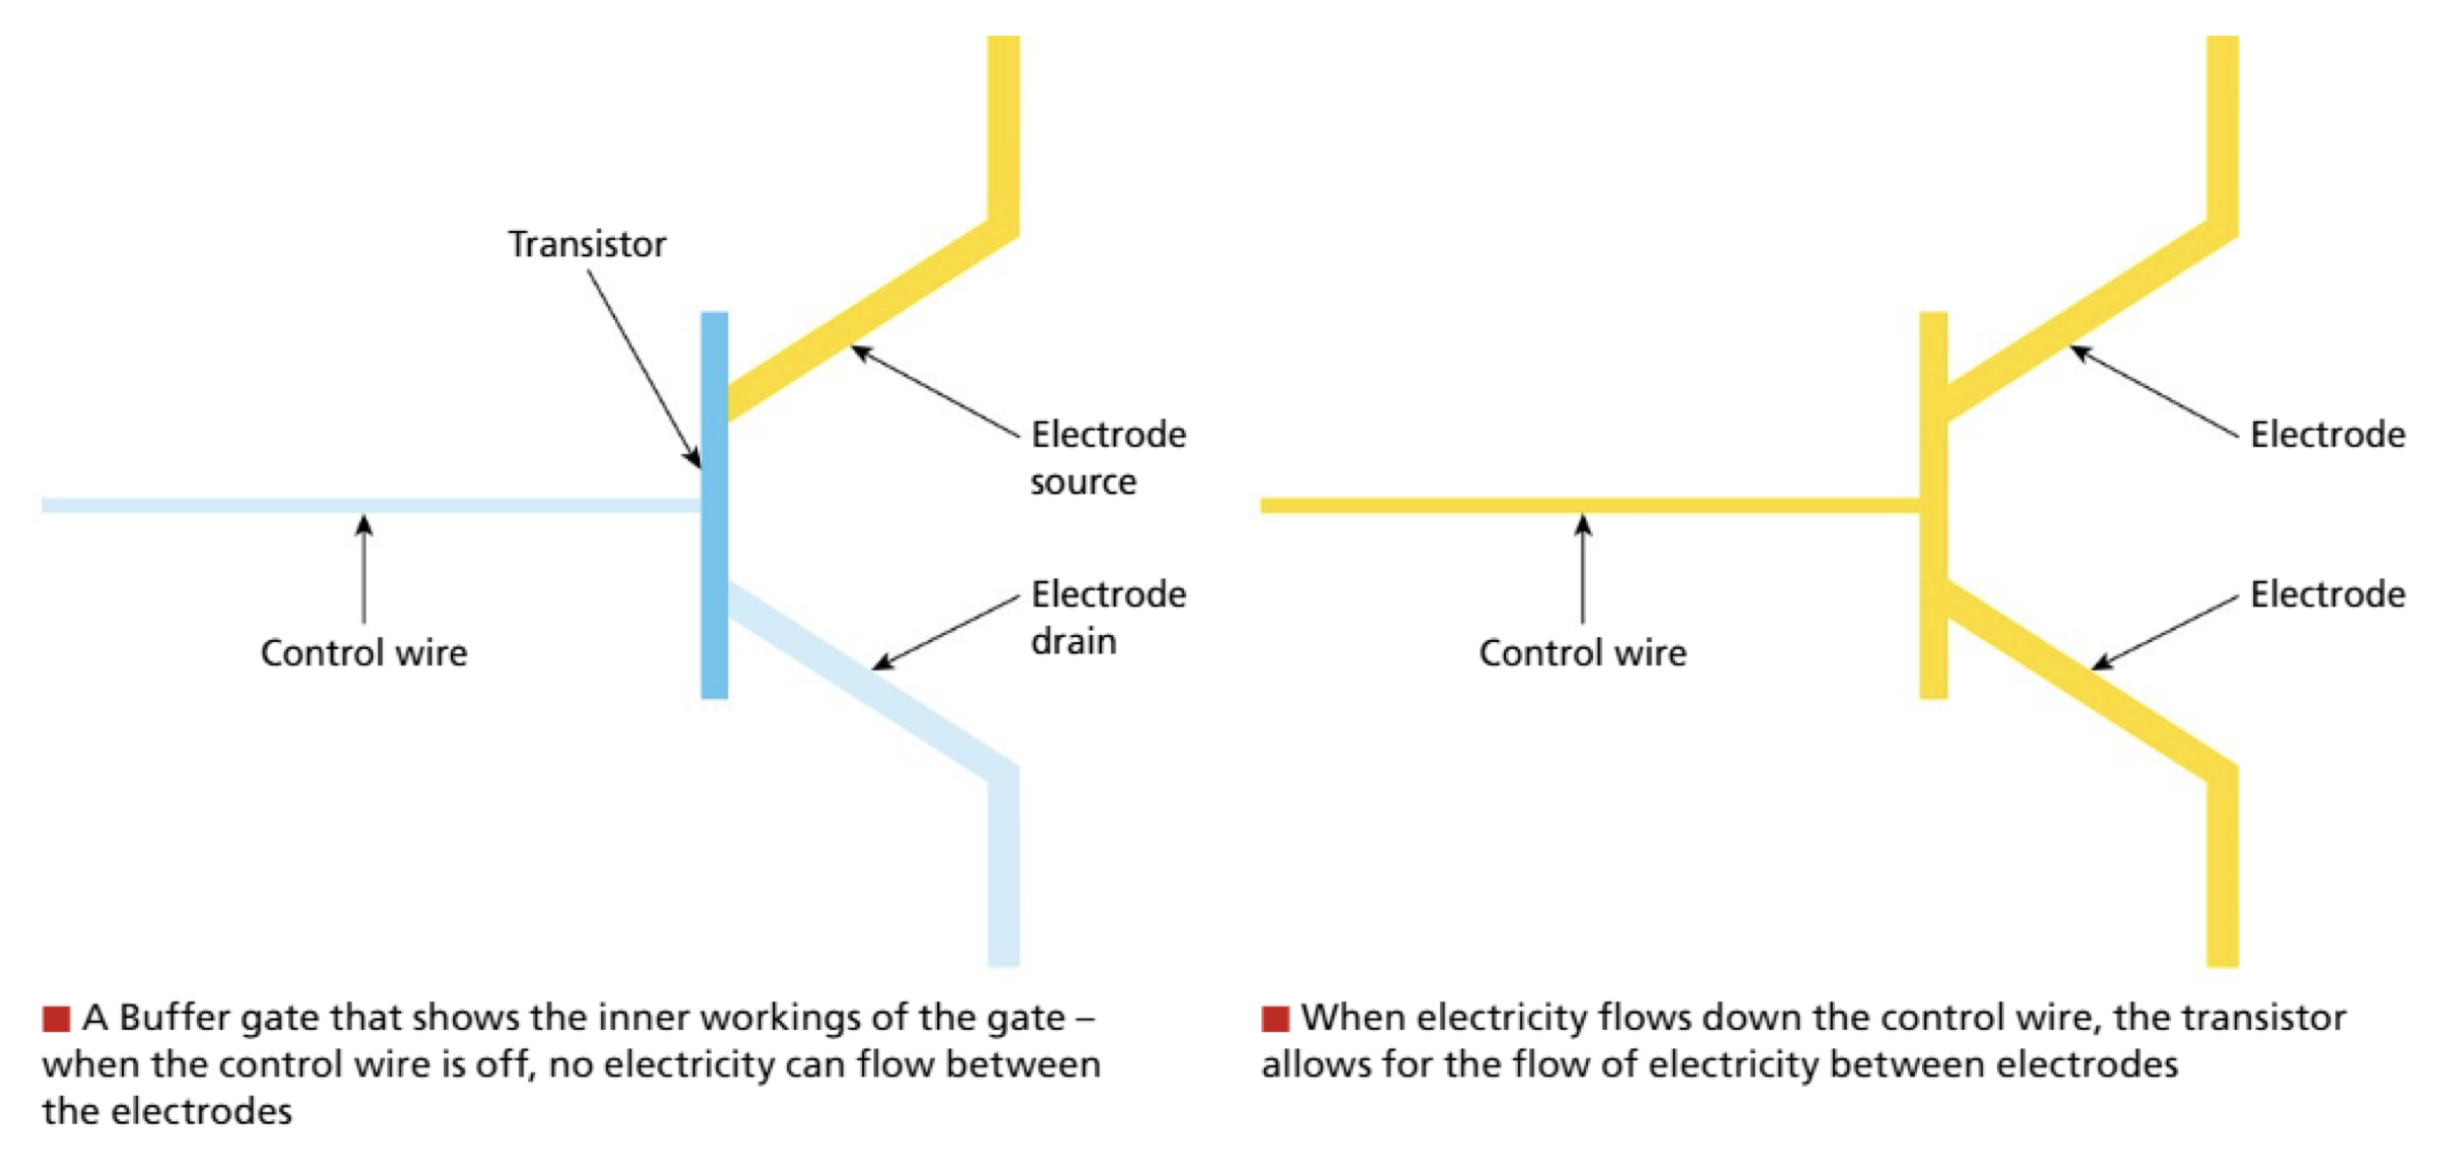
\includegraphics[width=\linewidth]{Screenshot 2026-10-05 at 12.32.29.png}

\end{minipage}

\vspace{12mm}

% =========================
% NAND
% =========================
\begin{minipage}{0.22\textwidth}
\centering
\begin{circuitikz}
    \node[nand port] (G) {};
    \draw (G.in 1) -- ++(-0.6,0);
    \draw (G.in 2) -- ++(-0.6,0);
    \draw (G.out) -- ++(0.6,0);
\end{circuitikz}

\vspace{3mm}

\textbf{NAND}

$Y = \overline{A \cdot B}$

\[
\begin{array}{cc|c}
A & B & Y \\ \hline
0 & 0 & 1 \\
0 & 1 & 1 \\
1 & 0 & 1 \\
1 & 1 & 0
\end{array}
\]

\end{minipage}
\hfill
% =========================
% NOR
% =========================
\begin{minipage}{0.22\textwidth}
\centering
\begin{circuitikz}
    \node[nor port] (G) {};
    \draw (G.in 1) -- ++(-0.6,0);
    \draw (G.in 2) -- ++(-0.6,0);
    \draw (G.out) -- ++(0.6,0);
\end{circuitikz}

\vspace{3mm}

\textbf{NOR}

$Y = \overline{A + B}$

\[
\begin{array}{cc|c}
A & B & Y \\ \hline
0 & 0 & 1 \\
0 & 1 & 0 \\
1 & 0 & 0 \\
1 & 1 & 0
\end{array}
\]

\end{minipage}
\hfill
% =========================
% XOR
% =========================
\begin{minipage}{0.22\textwidth}
\centering
\begin{circuitikz}
    \node[xor port] (G) {};
    \draw (G.in 1) -- ++(-0.6,0);
    \draw (G.in 2) -- ++(-0.6,0);
    \draw (G.out) -- ++(0.6,0);
\end{circuitikz}

\vspace{3mm}

\textbf{XOR}

$Y = A \oplus B$

\[
\begin{array}{cc|c}
A & B & Y \\ \hline
0 & 0 & 0 \\
0 & 1 & 1 \\
1 & 0 & 1 \\
1 & 1 & 0
\end{array}
\]

\end{minipage}
\hfill
% =========================
% XNOR
% =========================
\begin{minipage}{0.22\textwidth}
\centering
\begin{circuitikz}
    \node[xnor port] (G) {};
    \draw (G.in 1) -- ++(-0.6,0);
    \draw (G.in 2) -- ++(-0.6,0);
    \draw (G.out) -- ++(0.6,0);
\end{circuitikz}

\vspace{3mm}

\textbf{XNOR}

$Y = \overline{A \oplus B}$

\[
\begin{array}{cc|c}
A & B & Y \\ \hline
0 & 0 & 1 \\
0 & 1 & 0 \\
1 & 0 & 0 \\
1 & 1 & 1
\end{array}
\]

\end{minipage}

\end{center}

\paragraph{Constructing and analysing truth tables}
Starting with the intermediate values, work through the logic circuit. \\
Number of rows in truth table: $2^\text{\# of inputs}$\\
\textbf{Worked example: four inputs, all eight gate types.}\\
Each gate output is labelled; every label becomes a column of the truth table.
\[
\begin{aligned}
T_1 &= \operatorname{BUF}(A) = A &&\text{(BUFFER)}\\
T_2 &= \overline{T_1} = \overline{A} &&\text{(NOT)}\\
T_3 &= T_2 \cdot B = \overline{A}\,B &&\text{(AND)}\\
T_4 &= T_3 + C = \overline{A}\,B + C &&\text{(OR)}\\
T_5 &= T_4 \oplus D = (\overline{A}\,B + C)\oplus D &&\text{(XOR)}\\
T_6 &= \overline{T_5 \cdot B} &&\text{(NAND)}\\
T_7 &= \overline{T_6 + C} &&\text{(NOR)}\\
Y   &= \overline{T_7 \oplus D} &&\text{(XNOR)}
\end{aligned}
\]
Standard gate operators
$X\uparrow Y=\overline{X\cdot Y}$ (NAND), $X\downarrow Y=\overline{X+Y}$ (NOR)
and $X\odot Y=\overline{X\oplus Y}$ (XNOR),
\[
Y=\Big(\big(((\overline{A}\cdot B)+C)\oplus D\big)\uparrow B\Big)\downarrow C\ \odot\ D .
\]
\begin{center}
\resizebox{0.99\linewidth}{!}{%
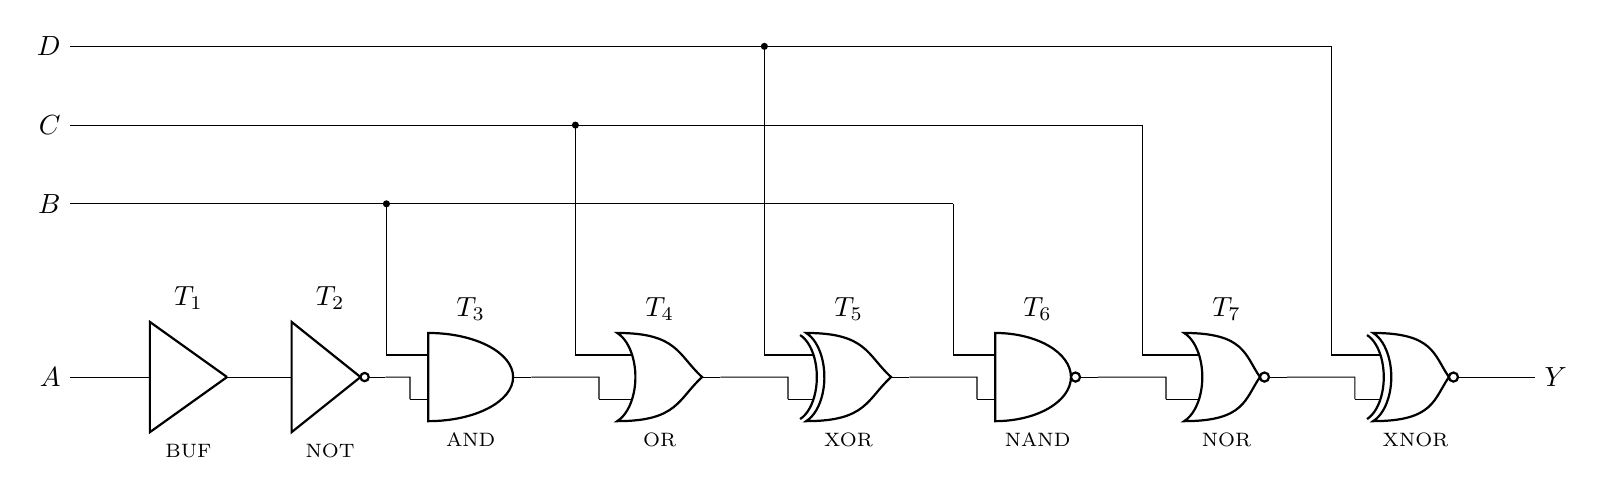
\begin{tikzpicture}
% ---- gates ----
\node[buffer port] (T1) at (0,0) {};
\node[not port]    (T2) at (1.8,0) {};
\node[and port]    (T3) at (4.2,0) {};
\node[or port]     (T4) at (6.6,0) {};
\node[xor port]    (T5) at (9.0,0) {};
\node[nand port]   (T6) at (11.4,0) {};
\node[nor port]    (T7) at (13.8,0) {};
\node[xnor port]   (TY) at (16.2,0) {};
% ---- input taps above (B, C and D buses) ----
\draw (-1.5,2.2) -- (9.714,2.2);
\draw (2.514,2.2) -- (2.514,0.28) -- (2.814,0.28);
\draw (9.714,2.2) -- (9.714,0.28) -- (10.014,0.28);
\fill (2.514,2.2) circle (0.045);
\draw (-1.5,3.2) -- (12.114,3.2);
\draw (4.914,3.2) -- (4.914,0.28) -- (5.214,0.28);
\draw (12.114,3.2) -- (12.114,0.28) -- (12.414,0.28);
\fill (4.914,3.2) circle (0.045);
\draw (-1.5,4.2) -- (14.514,4.2);
\draw (7.314,4.2) -- (7.314,0.28) -- (7.614,0.28);
\draw (14.514,4.2) -- (14.514,0.28) -- (14.814,0.28);
\fill (7.314,4.2) circle (0.045);
% ---- input A ----
\draw (-1.5,0) -- (T1.in);
\node[left] at (-1.5,0) {$A$};
\node[left] at (-1.5,2.2) {$B$};
\node[left] at (-1.5,3.2) {$C$};
\node[left] at (-1.5,4.2) {$D$};
% ---- signal chain ----
\draw (T1.out) -- (T2.in);
\draw (T2.out) -- (2.814,0) -- (T3.in 2);
\draw (T3.out) -- (5.214,0) -- (T4.in 2);
\draw (T4.out) -- (7.614,0) -- (T5.in 2);
\draw (T5.out) -- (10.014,0) -- (T6.in 2);
\draw (T6.out) -- (12.414,0) -- (T7.in 2);
\draw (T7.out) -- (14.814,0) -- (TY.in 2);
\draw (TY.out) -- (17.1,0) node[right] {$Y$};
% ---- labels ----
\node[above=1pt] at (T1.north) {$T_1$};
\node[above=1pt] at (T2.north) {$T_2$};
\node[above=1pt] at (T3.north) {$T_3$};
\node[above=1pt] at (T4.north) {$T_4$};
\node[above=1pt] at (T5.north) {$T_5$};
\node[above=1pt] at (T6.north) {$T_6$};
\node[above=1pt] at (T7.north) {$T_7$};
\node[below=1pt] at (T1.south) {\scriptsize BUF};
\node[below=1pt] at (T2.south) {\scriptsize NOT};
\node[below=1pt] at (T3.south) {\scriptsize AND};
\node[below=1pt] at (T4.south) {\scriptsize OR};
\node[below=1pt] at (T5.south) {\scriptsize XOR};
\node[below=1pt] at (T6.south) {\scriptsize NAND};
\node[below=1pt] at (T7.south) {\scriptsize NOR};
\node[below=1pt] at (TY.south) {\scriptsize XNOR};
\end{tikzpicture}}
\end{center}
\begin{center}
\renewcommand{\arraystretch}{1.12}
\begin{tabular}{cccc|ccccccc|c}
\toprule
\multicolumn{4}{c|}{Inputs} & \multicolumn{7}{c|}{Intermediate values} & Output \\
\cmidrule(lr){1-4}\cmidrule(lr){5-11}\cmidrule(lr){12-12}
$A$ & $B$ & $C$ & $D$ & $T_1$ & $T_2$ & $T_3$ & $T_4$ & $T_5$ & $T_6$ & $T_7$ & $Y$ \\
{\scriptsize} & {\scriptsize} & {\scriptsize} & {\scriptsize} & \scriptsize BUF & \scriptsize NOT & \scriptsize AND & \scriptsize OR & \scriptsize XOR & \scriptsize NAND & \scriptsize NOR & \scriptsize XNOR \\
\midrule
0 & 0 & 0 & 0 & 0 & 1 & 0 & 0 & 0 & 1 & 0 & 1 \\
0 & 0 & 0 & 1 & 0 & 1 & 0 & 0 & 1 & 1 & 0 & 0 \\
0 & 0 & 1 & 0 & 0 & 1 & 0 & 1 & 1 & 1 & 0 & 1 \\
0 & 0 & 1 & 1 & 0 & 1 & 0 & 1 & 0 & 1 & 0 & 0 \\
0 & 1 & 0 & 0 & 0 & 1 & 1 & 1 & 1 & 0 & 1 & 0 \\
0 & 1 & 0 & 1 & 0 & 1 & 1 & 1 & 0 & 1 & 0 & 0 \\
0 & 1 & 1 & 0 & 0 & 1 & 1 & 1 & 1 & 0 & 0 & 1 \\
0 & 1 & 1 & 1 & 0 & 1 & 1 & 1 & 0 & 1 & 0 & 0 \\
1 & 0 & 0 & 0 & 1 & 0 & 0 & 0 & 0 & 1 & 0 & 1 \\
1 & 0 & 0 & 1 & 1 & 0 & 0 & 0 & 1 & 1 & 0 & 0 \\
1 & 0 & 1 & 0 & 1 & 0 & 0 & 1 & 1 & 1 & 0 & 1 \\
1 & 0 & 1 & 1 & 1 & 0 & 0 & 1 & 0 & 1 & 0 & 0 \\
1 & 1 & 0 & 0 & 1 & 0 & 0 & 0 & 0 & 1 & 0 & 1 \\
1 & 1 & 0 & 1 & 1 & 0 & 0 & 0 & 1 & 0 & 1 & 1 \\
1 & 1 & 1 & 0 & 1 & 0 & 0 & 1 & 1 & 0 & 0 & 1 \\
1 & 1 & 1 & 1 & 1 & 0 & 0 & 1 & 0 & 1 & 0 & 0 \\
\bottomrule
\end{tabular}
\end{center}
Truth tables to determine outputs from inputs for a problem description: With a problem description, we first need to identify the inputs. Here we have three: alarm switch, baby crying and room temperature, which we can represent as A, B and C and set up our truth table. \\\\
Logical expressions: We can represent logic circuits using Boolean algebra. In Boolean algebra, parentheses are often used to indicate which operations should be 
performed first. If no parentheses are present, follow this sequence: NOT, AND, OR.\\\\
\textbf{Karnaugh maps and algebraic simplification}\\
Two input K-map: the four cells hold the output for the four possible combinations of $A$ and $B$. For example, the function $F=A+B$ gives
\begin{center}
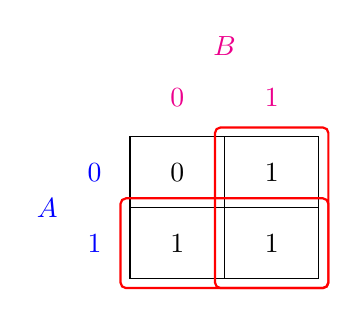
\begin{tikzpicture}[font=\normalsize]
  \draw (0,0) rectangle (2.4,-1.8);
  \draw (1.2,0) -- (1.2,-1.8);
  \draw (0,-0.9) -- (2.4,-0.9);
  \node at (0.6,-0.45) {0};
  \node at (1.8,-0.45) {1};
  \node at (0.6,-1.35) {1};
  \node at (1.8,-1.35) {1};
  \node[text=magenta] at (0.6,0.5) {0};
  \node[text=magenta] at (1.8,0.5) {1};
  \node[text=magenta] at (1.2,1.15) {$B$};
  \node[text=blue] at (-0.45,-0.45) {0};
  \node[text=blue] at (-0.45,-1.35) {1};
  \node[text=blue] at (-1.05,-0.9) {$A$};
  \draw[red, thick, rounded corners=2pt] (1.08,0.12) rectangle (2.52,-1.92);
  \draw[red, thick, rounded corners=2pt] (-0.12,-0.78) rectangle (2.52,-1.92);
\end{tikzpicture}
\end{center}
The two 1s in the column $B=1$ group to give $B$, and the two 1s in the row $A=1$ group to give $A$, so the K-map simplifies to $F=A+B$.\\\\
Three input K-map: the eight cells hold the output for the eight combinations of $A$, $B$ and $C$, with the column labels in Gray-code order $00,01,11,10$ so that adjacent cells differ by one variable. For example, the function $F=AB+C$ gives
\begin{center}
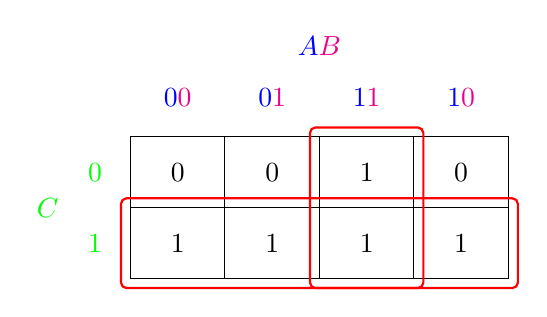
\begin{tikzpicture}[font=\normalsize]
  \draw (0,0) rectangle (4.8,-1.8);
  \draw (1.2,0) -- (1.2,-1.8);
  \draw (2.4,0) -- (2.4,-1.8);
  \draw (3.6,0) -- (3.6,-1.8);
  \draw (0,-0.9) -- (4.8,-0.9);
  \node at (0.6,-0.45) {0};
  \node at (1.8,-0.45) {0};
  \node at (3.0,-0.45) {1};
  \node at (4.2,-0.45) {0};
  \node at (0.6,-1.35) {1};
  \node at (1.8,-1.35) {1};
  \node at (3.0,-1.35) {1};
  \node at (4.2,-1.35) {1};
  \node at (0.6,0.5) {\textcolor{blue}{0}\textcolor{magenta}{0}};
  \node at (1.8,0.5) {\textcolor{blue}{0}\textcolor{magenta}{1}};
  \node at (3.0,0.5) {\textcolor{blue}{1}\textcolor{magenta}{1}};
  \node at (4.2,0.5) {\textcolor{blue}{1}\textcolor{magenta}{0}};
  \node at (2.4,1.15) {\textcolor{blue}{$A$}\textcolor{magenta}{$B$}};
  \node[text=green] at (-0.45,-0.45) {0};
  \node[text=green] at (-0.45,-1.35) {1};
  \node[text=green] at (-1.05,-0.9) {$C$};
  \draw[red, thick, rounded corners=2pt] (-0.12,-0.78) rectangle (4.92,-1.92);
  \draw[red, thick, rounded corners=2pt] (2.28,0.12) rectangle (3.72,-1.92);
\end{tikzpicture}
\end{center}
The four 1s in the row $C=1$ (that is, all four columns) group to give $C$, and the two 1s in the column $AB=11$ (that is, $C=0$ and $C=1$) group to give $AB$, so the K-map simplifies to $F=AB+C$.\\\\
Another three input K-map: the function $F=\overline{A}BC+A\overline{B}C+ABC$ gives
\begin{center}
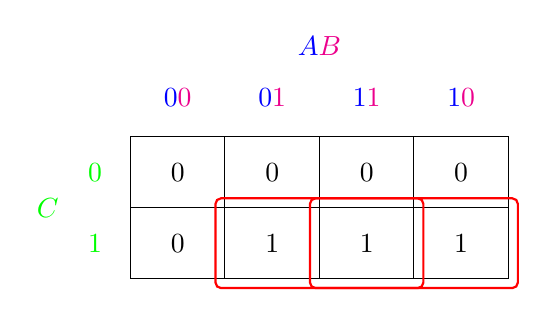
\begin{tikzpicture}[font=\normalsize]
  \draw (0,0) rectangle (4.8,-1.8);
  \draw (1.2,0) -- (1.2,-1.8);
  \draw (2.4,0) -- (2.4,-1.8);
  \draw (3.6,0) -- (3.6,-1.8);
  \draw (0,-0.9) -- (4.8,-0.9);
  \node at (0.6,-0.45) {0};
  \node at (1.8,-0.45) {0};
  \node at (3.0,-0.45) {0};
  \node at (4.2,-0.45) {0};
  \node at (0.6,-1.35) {0};
  \node at (1.8,-1.35) {1};
  \node at (3.0,-1.35) {1};
  \node at (4.2,-1.35) {1};
  \node at (0.6,0.5) {\textcolor{blue}{0}\textcolor{magenta}{0}};
  \node at (1.8,0.5) {\textcolor{blue}{0}\textcolor{magenta}{1}};
  \node at (3.0,0.5) {\textcolor{blue}{1}\textcolor{magenta}{1}};
  \node at (4.2,0.5) {\textcolor{blue}{1}\textcolor{magenta}{0}};
  \node at (2.4,1.15) {\textcolor{blue}{$A$}\textcolor{magenta}{$B$}};
  \node[text=green] at (-0.45,-0.45) {0};
  \node[text=green] at (-0.45,-1.35) {1};
  \node[text=green] at (-1.05,-0.9) {$C$};
  \draw[red, thick, rounded corners=2pt] (1.08,-0.78) rectangle (3.72,-1.92);
  \draw[red, thick, rounded corners=2pt] (2.28,-0.78) rectangle (4.92,-1.92);
\end{tikzpicture}
\end{center}
The two 1s in the row $C=1$ with $B=1$ (that is, $01$ and $11$) group to give $BC$, and the two 1s in the row $C=1$ with $A=1$ (that is, $11$ and $10$) group to give $AC$, so the K-map simplifies to $F=BC+AC$.\\\\
\textbf{Grouping conventions}
\begin{itemize}
    \item Groups must contain powers of 2: One, two, four, eight or sixteen 1s can be 
grouped together.
	\item Groups must be rectangular or square: Each group should form a rectangle or 
square shape. 
\item Groups cannot be diagonal: Adjacent 1s can only be grouped horizontally or vertically, 
not diagonally. 
\item Groups must be as large as possible: Always aim to make the largest groups to simplify the expression further. 
\item Groups can overlap: Some 1s may be included in more than one group if it helps form 
larger groups. 
\item Minimize the total number of groups: The goal is to use the smallest number of groups to cover all the 1s. 
    \end{itemize}
To determine the expression from the groups, we look at each group of cells and refer to the 
variables. If a variable’s value stays the same across all the cells in the group, we keep that 
variable in the simplified expression. Iowever, if the variable’s value changes across the group, we discard it from the expression. \\\\
\textbf{Wrapping around edges in K-maps}\\
K-maps are considered three-dimensional, and groups can be formed from left 
to right and top to bottom (although only left to right is possible with three inputs).
In the example of $F=\overline{B}+ABC$:
\begin{center}
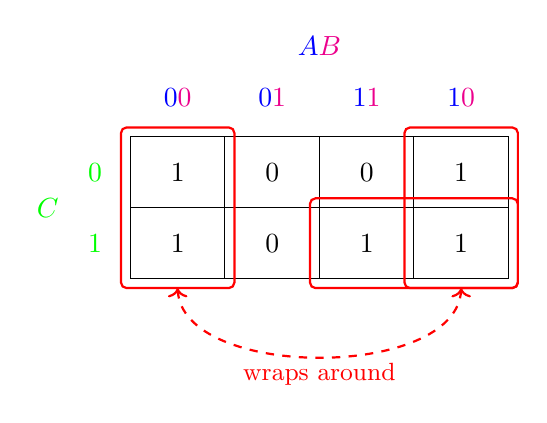
\begin{tikzpicture}[font=\normalsize]
  \draw (0,0) rectangle (4.8,-1.8);
  \draw (1.2,0) -- (1.2,-1.8);
  \draw (2.4,0) -- (2.4,-1.8);
  \draw (3.6,0) -- (3.6,-1.8);
  \draw (0,-0.9) -- (4.8,-0.9);
  \node at (0.6,-0.45) {1};
  \node at (1.8,-0.45) {0};
  \node at (3.0,-0.45) {0};
  \node at (4.2,-0.45) {1};
  \node at (0.6,-1.35) {1};
  \node at (1.8,-1.35) {0};
  \node at (3.0,-1.35) {1};
  \node at (4.2,-1.35) {1};
  \node at (0.6,0.5) {\textcolor{blue}{0}\textcolor{magenta}{0}};
  \node at (1.8,0.5) {\textcolor{blue}{0}\textcolor{magenta}{1}};
  \node at (3.0,0.5) {\textcolor{blue}{1}\textcolor{magenta}{1}};
  \node at (4.2,0.5) {\textcolor{blue}{1}\textcolor{magenta}{0}};
  \node at (2.4,1.15) {\textcolor{blue}{$A$}\textcolor{magenta}{$B$}};
  \node[text=green] at (-0.45,-0.45) {0};
  \node[text=green] at (-0.45,-1.35) {1};
  \node[text=green] at (-1.05,-0.9) {$C$};
  \draw[red, thick, rounded corners=2pt] (-0.12,0.12) rectangle (1.32,-1.92);
  \draw[red, thick, rounded corners=2pt] (3.48,0.12) rectangle (4.92,-1.92);
  \draw[red, thick, dashed, {<->}] (0.6,-1.92) .. controls (0.6,-3.1) and (4.2,-3.1) .. (4.2,-1.92);
  \node[red, font=\small] at (2.4,-3.02) {wraps around};
  \draw[red, thick, rounded corners=2pt] (2.28,-0.78) rectangle (4.92,-1.92);
\end{tikzpicture}
\end{center}
The four 1s in the columns $AB=00$ and $AB=10$ wrap around the left and right edges to form one group of four in which $B=0$ throughout, giving $\overline{B}$; the remaining 1 groups with the adjacent 1 in $AB=10$ (overlapping the $\overline{B}$ group) to give $AC$, so the K-map simplifies to $F=\overline{B}+AC$.
\\\\
Four-variable K-maps wrap in both directions, so the map behaves like a torus: the left and right edges join, and the top and bottom edges join as well. The figure shows a $4\times4$ map and the same map drawn on a torus; the four wrapping corner cells are marked with dots.
\begin{center}
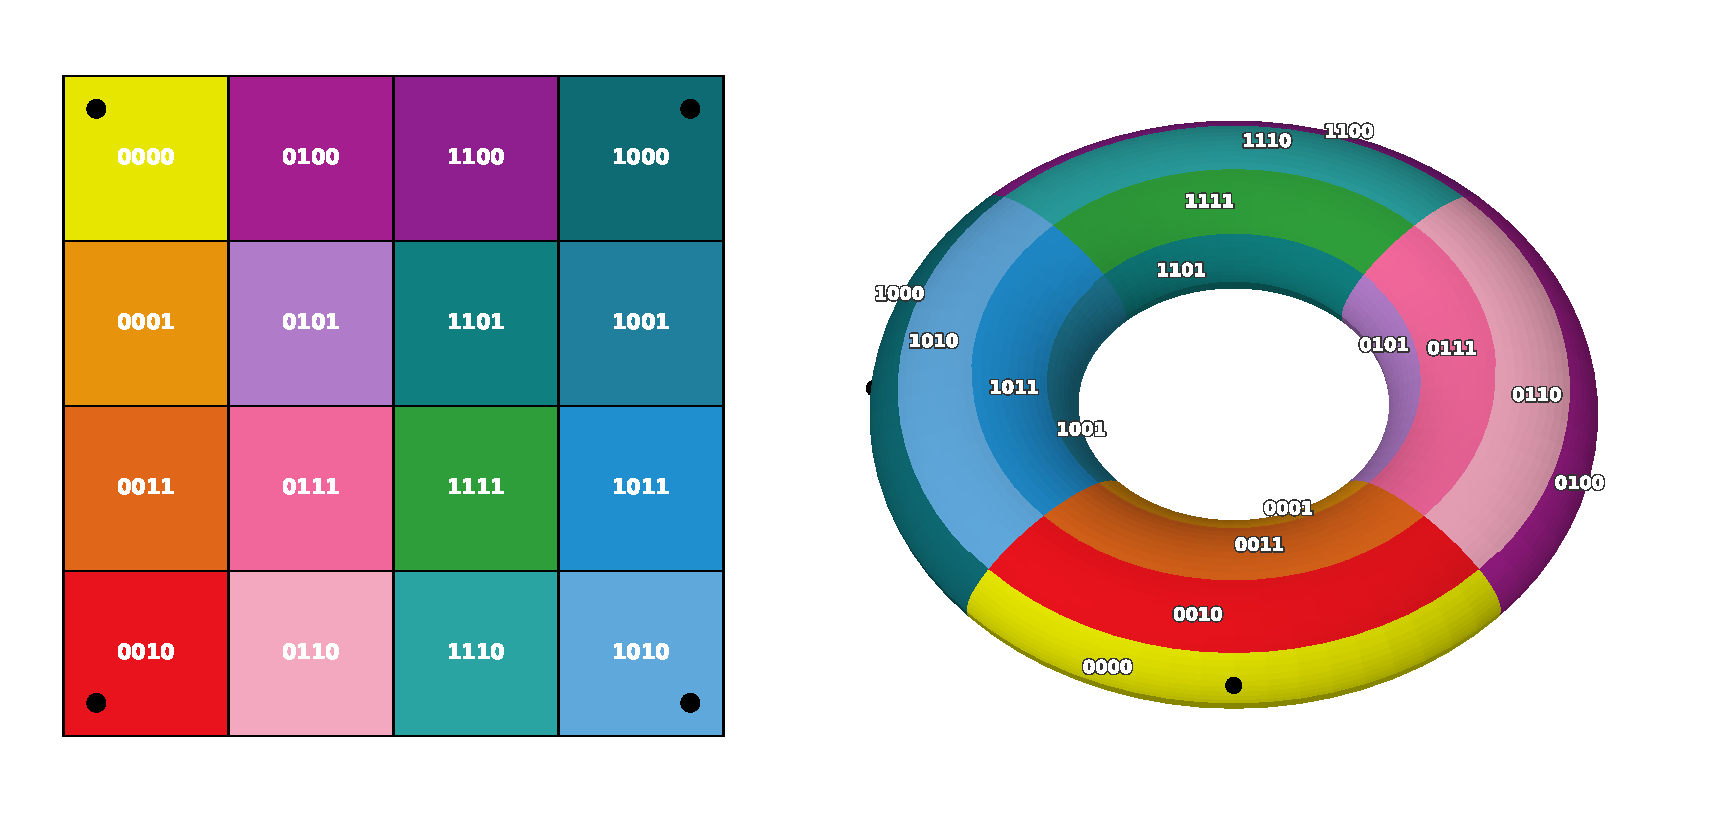
\includegraphics[width=0.95\linewidth]{kmap-torus.pdf}
\end{center}
\paragraph{Constructing logic diagrams}
By understanding the principles of Boolean algebra, we can simplify complex logic expressions and translate them into circuit diagrams. This journey from abstract mathematical notation 
to circuit design is essential for creating efficient and reliable digital systems. When a logic expression is given, follow the conventional operation sequence (parentheses first, then NOT, AND, OR...) 
\subsubsection{Operating systems and control systems}
\paragraph{The role of operating systems}
An operating system (OS) is the fundamental software that manages computer hardware 
and software resources and provides common services for computer programs. It acts as an intermediary between the user and the computer hardware, ensuring efficient and secure operation of the system. Operating systems simplify user interactions with computer hardware by \textbf{abstraction}: users and applications do not need to understand the detailed workings of components such as CPUs, memory and I/O devices, because the OS provides a set of high-level services and interfaces that hide these complexities, making the system easier to use and to program.
\begin{itemize}
    \item CPU management: allocating CPU time to various processes and ensuring 
efficient execution 
	\item Memory management: handling the allocation and de-allocation of memory to 
applications, and managing virtual memory to extend physical memory capacity 
\item Storage management: organizing and managing data on storage devices, ensuring reliable data storage and retrieval 
\item Device management: controlling and co-ordinating hardware devices, providing drivers and interfaces for seamless operation. 
\end{itemize}
\paragraph{Functions of an operating system}
\begin{itemize}
    \item Memory management: control and coordination of a computer's primary memory; the OS ensures that memory is allocated efficiently to processes and applications, maintains system stability and protects memory areas from unauthorized access. When an app is opened, the OS will load it into RAM. How the memory allocation mechanism works:
    \begin{enumerate}
        \item Locate the app on the storage device and read the executable file, containing all the app's code and initial data. 
        \item The OS then allocates the necessary memory space for the application. This includes space for the code, data and any other required resources. The OS ensures that the application has enough space to execute without interfering with other processes. 
        \item Once the application is loaded into RAM, the OS continuously manages memory to ensure efficient operation and system stability.
        \begin{enumerate}
            \item While the application is running, the OS can dynamically allocate and de-allocate memory as needed by the application. 
            \item The OS also ensures that each process operates within its own memory space. This prevents processes from interfering with each other, which enhances the security and stability of the system. 
            \item If the applications require more memory than is available in the RAM, the OS can use virtual memory to keep the system running smoothly. (Virtual memory: a memory-management technique that allows a computer to use more memory than what's physically available by temporarily transferring data from RAM to disk storage, enabling the execution of larger programs and multitasking.) This is not ideal, since reading from a storage device is much slower than accessing RAM, but by switching higher-priority processes into RAM and lower-priority ones into virtual memory, the OS keeps the whole system running at an optimal level.
            \end{enumerate}
    \end{enumerate}
\begin{center}
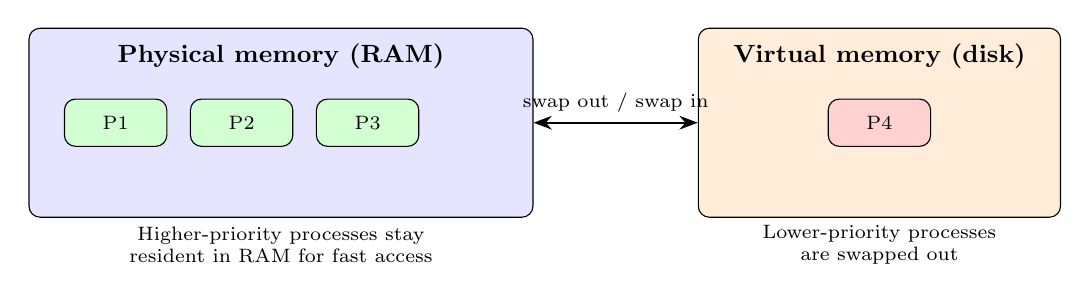
\begin{tikzpicture}[font=\scriptsize,>=Stealth]
\node[draw,rounded corners,fill=blue!10,minimum width=6.4cm,minimum height=2.4cm] (ram) at (0,0) {};
\node[font=\small\bfseries] at (0,0.85) {Physical memory (RAM)};
\node[draw,rounded corners,fill=green!18,minimum width=1.3cm,minimum height=0.6cm] (p1) at (-2.1,0) {P1};
\node[draw,rounded corners,fill=green!18,minimum width=1.3cm,minimum height=0.6cm] (p2) at (-0.5,0) {P2};
\node[draw,rounded corners,fill=green!18,minimum width=1.3cm,minimum height=0.6cm] (p3) at (1.1,0) {P3};
\node[font=\scriptsize,align=center,text width=6.2cm] at (0,-1.55) {Higher-priority processes stay resident in RAM for fast access};
\node[draw,rounded corners,fill=orange!15,minimum width=4.6cm,minimum height=2.4cm] (disk) at (7.6,0) {};
\node[font=\small\bfseries] at (7.6,0.85) {Virtual memory (disk)};
\node[draw,rounded corners,fill=red!18,minimum width=1.3cm,minimum height=0.6cm] (p4) at (7.6,0) {P4};
\node[font=\scriptsize,align=center,text width=4.4cm] at (7.6,-1.55) {Lower-priority processes are swapped out};
\draw[<->,thick] (ram.east) -- node[above,font=\scriptsize]{swap out / swap in} (disk.west);
\end{tikzpicture}
\end{center}
    \item File management: involving the storage, retrieval, organization and manipulation of data on storage devices. The OS provides a structured way to manage files and directories, ensuring system stability and security. 
    \begin{enumerate}
        \item The OS employs a hierarchical file system to organize files in a logical and structured manner. Files are organized into directories (or folders), which can contain further directories, creating a tree-like structure. This organization makes it easier for users and applications to locate and manage data. 
        \item The OS allows a number of set file operations that users and applications can perform on the files and directories, including creating new files and directories; reading and writing data to files; deleting files; renaming files; and moving or copying files and directories to different locations. 
        \item To ensure consistency and avoid conflicts, the OS enforces rules for naming files, ensuring no two files in the same directory have the same name. Files often have a \textbf{file extension} --- a suffix at the end of the filename that indicates the file type and the program associated with opening or processing that file (e.g.\ .jpg for images, .exe for applications) --- although, depending on the OS settings, these may be hidden from the user.
        \item When managing the storage of files, the OS uses various methods to improve performance: how it allocates files on the physical storage medium, manages free space, and performs maintenance on the saved data.
        \item \textbf{Fragmentation} occurs over time as files are created, modified and deleted, causing them to be scattered across different sectors of the disk. \textbf{Defragmentation} is the process of reorganizing the data on a hard drive so that files are stored in contiguous blocks, reducing fragmentation and improving access speed and overall system performance.
    \end{enumerate}
    \item Device management: ensuring that hardware devices operate efficiently and interact seamlessly with software applications.
    \begin{enumerate}
        \item The OS controls and co-ordinates the use of hardware components such as printers, disk drives, display screens, keyboards and network interfaces through specialized software called device drivers. (specialized software programs that allow the operating system to communicate with and control hardware devices, e.g. printers, graphics cards or network adapters, by providing 
the necessary instructions and protocols. ) Each piece of hardware requires a specific driver to function correctly and efficiently, and the OS uses these drivers to provide a \textbf{uniform interface}, so that applications can interact with the hardware without needing to understand its specifics.
	\item The OS also handles input/output (I/O) management to co-ordinate data transfer between the computer and peripheral devices. It employs techniques such as buffering, caching and spooling to optimize performance and reliability.
	\begin{enumerate}
	    \item Buffering: the process of temporarily storing data in a memory area (buffer) while it is being transferred between two devices or processes, helping to manage differences in data-flow rates (accommodating speed differences between the CPU and peripheral devices) and ensuring smooth, uninterrupted operation.
	    \item Caching: the process of temporarily storing frequently accessed data in a high-speed storage area (cache) to reduce access time and improve system performance by enabling quicker retrieval of the data. 
	    \item Spooling: the process of queuing data or tasks in a buffer, typically for input / output devices such as printers, which cannot handle interleaved data streams, so that the data is processed sequentially and at the devices' own pace, allowing the system to continue working on other tasks in the meantime.
	    \end{enumerate}
        \item Modern operating systems have introduced user-friendly ways of connecting devices, such as Plug and Play (PnP) technology. With PnP, the OS can automatically identify a device that has been attached and install the necessary drivers and configure settings without the need for user interaction. The OS is also capable of detecting errors and taking action to recover from them, by resetting the device, reinitializing drivers or notifying the user of the issue. Additionally, the OS provides security and access control to ensure that only authorized users and processes can access certain devices, maintaining system integrity and security. 
    \end{enumerate}
\begin{center}
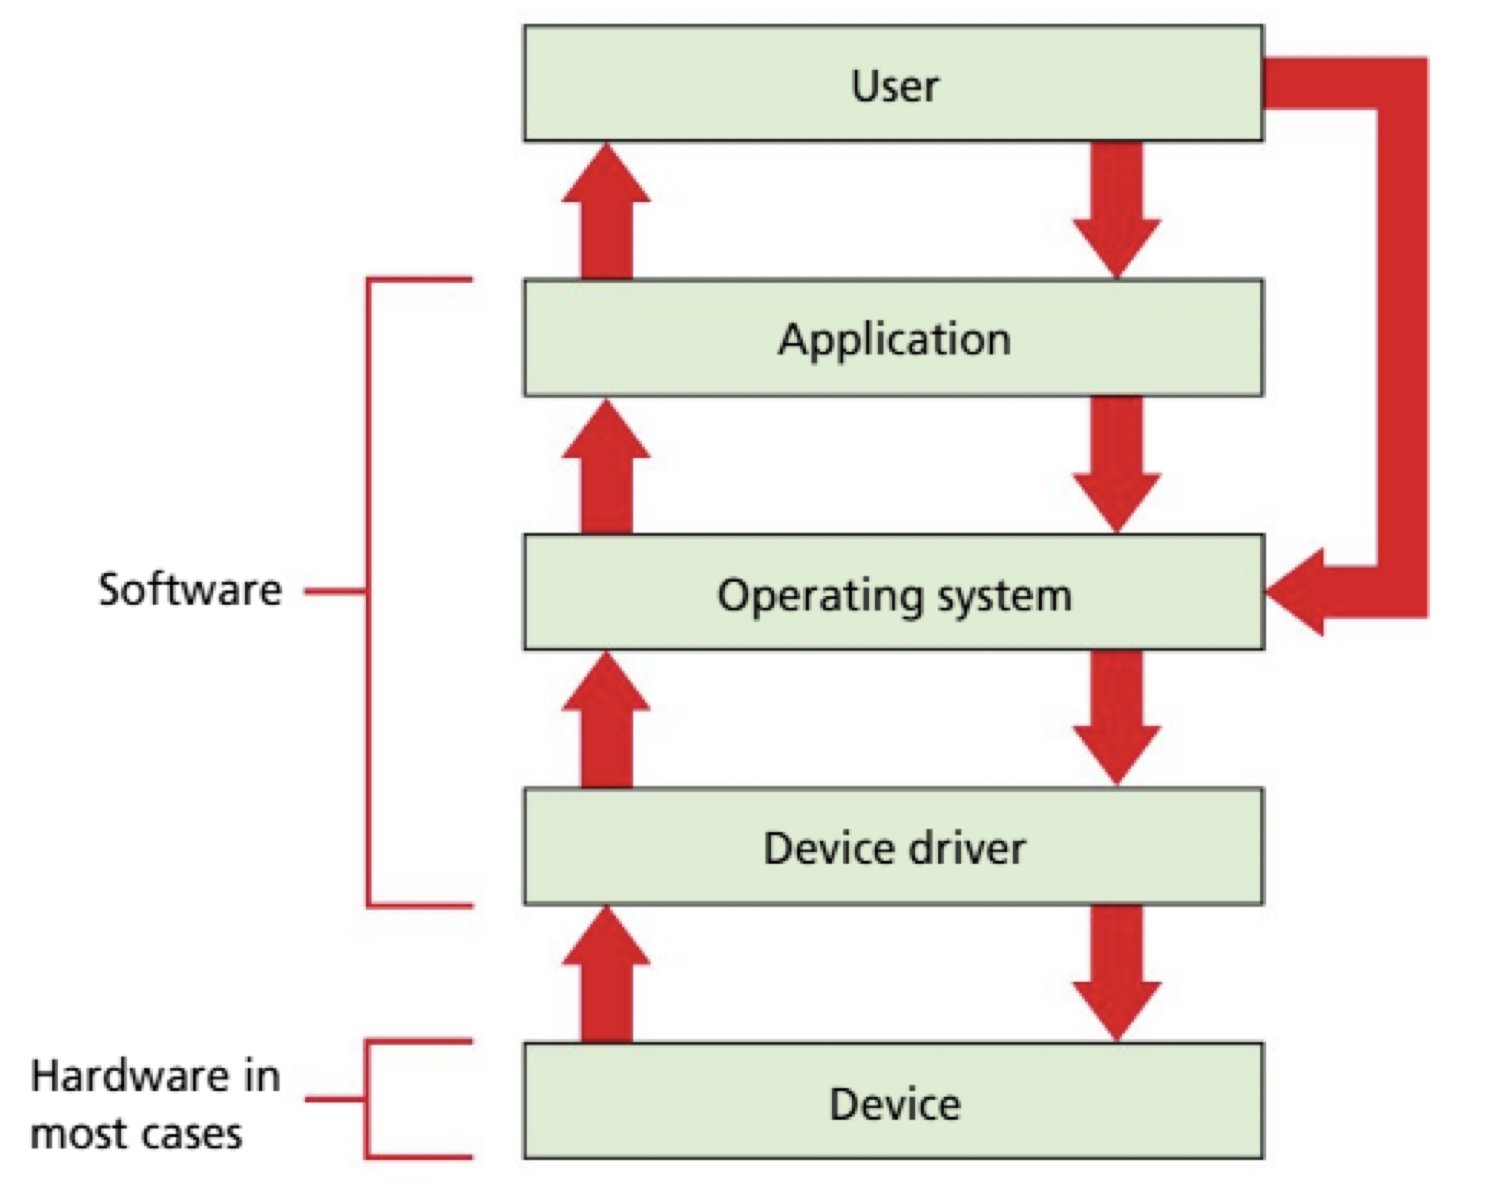
\includegraphics[width=0.6\linewidth]{Screenshot 2026-10-19 at 18.51.25.png}
\end{center}
    \item Scheduling: The OS schedules the process of managing the execution of multiple processes by determining which process runs at any given time. The scheduler is responsible for allocating CPU time to processes, ensuring efficient and fair use of system resources. This function is crucial for multitasking environments, where multiple applications and background processes run concurrently. By implementing various scheduling algorithms, the OS aims to optimize performance, reduce wait times and maintain system stability. 
    \item Security: OS security is designed to protect the integrity, confidentiality and availability of information and resources within the computer system. It has mechanisms to safeguard against threats, prevent unauthorized access and ensure that users and applications can operate securely.
    \begin{itemize}
        \item User authentication: User authentication can be used in multiple ways. Initially, the OS may require the user to
        authenticate themselves to log in to the system. It would require the user to provide credentials
        such as a username and password, biometric data or security tokens. (physical or digital
        devices that generate or store authentication credentials, such as one-time passwords or
        cryptographic keys, used to verify a user's identity and secure access to
        systems, networks or online services.) Once logged on, based on the user settings, the OS can then grant or prevent access to certain files, folders or
        applications on the system. This allows systems to have multiple users with different access
        credentials, such as an administrator and a standard user.
        \item Encryption: The OS can provide tools and frameworks for encrypting files, communication channels
and devices. The encryption ensures that the data, even if it is intercepted or accessed by
unauthorized individuals, cannot be read without the decryption key.
        \item Auditing and monitoring: All system activities, such as users logging in, file access, system errors and administrator
        actions, are tracked by the OS in a log. These logs are used for auditing and monitoring
        purposes and can help administrators detect suspicious activities and potential security
        breaches. They can also be used to help identify issues and areas for improving the
        system performance.
        \begin{center}
        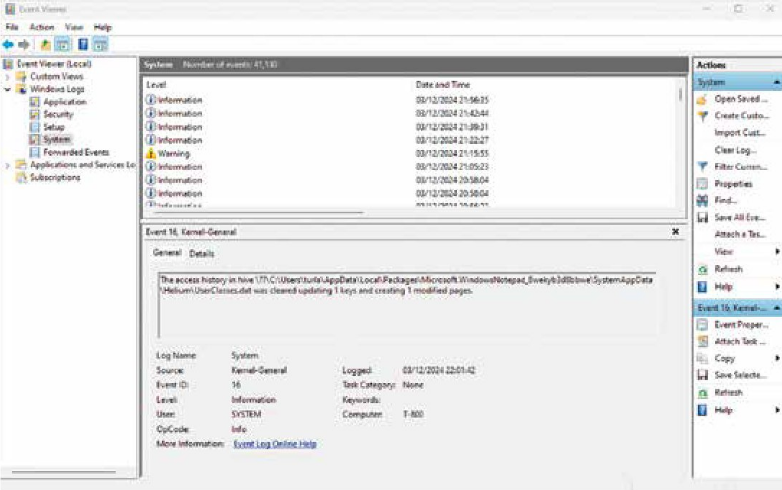
\includegraphics[width=0.72\linewidth]{textbook-event-viewer.png}\\
        {\footnotesize Windows Event Viewer: the OS records system events (logons, errors, service activity) so that they can be reviewed for auditing and monitoring.}
        \end{center}
        \item Malware protection: The OS includes mechanisms to detect and prevent malware infections and intruders. These
        include antivirus software, firewalls and intrusion detection systems (IDS). These tools scan
        for malicious software, monitor network traffic and block unauthorized access attempts,
        protecting the system from viruses, worms, trojans and other malicious threats. (\textbf{Malware}: a general term for any software designed with malicious intent, e.g.\ viruses, worms, trojans, spyware and ransomware, which can damage systems, steal data or disrupt operations. A \emph{virus} attaches itself to legitimate files or programs and spreads to other files or systems, often causing damage or disruption; a \emph{worm} self-replicates and spreads across networks without needing to attach to other programs, exploiting vulnerabilities to infect multiple systems; a \emph{trojan} appears legitimate but carries hidden malicious code, which can create backdoors, steal data or cause harm once the user executes it.)
        \end{itemize}
    \item Accounting: OS accounting functions are essential for monitoring and managing the usage of system resources. They track resource consumption by users and processes, providing valuable data for system administrators to analyse performance, allocate costs and optimize resource utilization.
    \begin{itemize}
        \item Resource usage tracking: The OS continuously monitors the consumption of various resources by users and 
processes; this includes tracking:
        \begin{itemize}
            \item CPU usage: the amount of CPU time consumed by each process or user.
            \item Memory usage: the amount of RAM allocated and used by each process.
            \item Disk usage: the amount of storage space occupied by the files and directories owned by each user.
            \item Network usage: the volume of data sent and received over the network by each process or user.
        \end{itemize}
        \item Process accounting: involves maintaining detailed records of each process that runs on the 
system; this includes information such as process ID, user ID, execution time, start and end times, resource consumption.
        \item User accounting: tracks the resource usage by individual users or user groups; this information is crucial for cost allocation (in multi-user environments such as universities or enterprises, usage data can be used to allocate costs to different departments or projects according to their consumption) and quota management (enforcing resource usage limits so that no single user monopolizes system resources, e.g.\ disk quotas and memory limits).
        \item Performance monitoring: The OS accounting functions are integral to performance monitoring; by analysing 
resource usage data, system administrators can identify bottlenecks (areas where resources are being overutilized, causing performance degradation), underutilizations (resources that are underused, indicating potential areas for optimization) and trends (patterns in resource usage over time, which can inform capacity planning and system upgrades).
        \item Auditing and reporting: The OS generates detailed reports based on the collected accounting data; these reports can be used for auditing (ensuring compliance with organizational policies and regulatory requirements by reviewing resource usage and access patterns), security analysis (detecting unusual or suspicious activity by analysing resource usage anomalies) and resource management (making informed decisions about resource allocation, system configuration and future investments).
        \item Billing and chargeback: In environments where resource usage needs to be billed to individual users or 
departments, such as cloud-computing services or academic institutions, OS accounting functions enable usage-based billing (charging users based on their actual consumption, such as CPU hours, memory usage and network bandwidth) and chargeback (allocating costs to different departments or projects according to their resource usage, promoting accountability and efficient resource use).
        \end{itemize}
    \item GUI: By offering visual elements such as windows, icons, menus and pointers, the OS provides a user-friendly environment for interacting with the computer and allows the user to execute commands, manage files and run applications. 
    \begin{itemize}
        \item User interface elements: The user interface elements provided by the OS allow the user to interact with the system intuitively.
        \begin{itemize}
            \item Windows display the contents of applications, documents or system information.
            \item Icons give a graphical representation to applications, files and system functions, providing quick access to frequently used items.
            \item Menus offer lists of commands or options to access various functions, making navigation and operation straightforward.
            \item Pointers, usually an arrow or cursor, are controlled with an input device such as a mouse, enabling users to select, drag and interact with GUI elements seamlessly.
        \end{itemize}
        \item Application management: The GUI facilitates the management of and interaction with multiple applications, enhancing user productivity and experience. Task switching lets users move quickly between open applications, with features like the taskbar or the application switcher (Alt + tab) enabling efficient navigation; window management helps users organize their workspace by arranging, overlapping and tiling windows, and snapping windows to edges or corners creates a split-screen effect for multitasking; the desktop environment, where users can place icons, shortcuts and widgets, allows for a personalized and organized workspace.
        \item File and system management: The GUI simplifies file and system management tasks through visual tools and interfaces. A GUI-based file management tool such as File Explorer allows users to navigate directories, view file properties and perform operations such as copying, moving, deleting and renaming files and folders, and often includes features such as search, sort and filter. The GUI also provides access to system settings and control panels, enabling users to configure hardware, software and system preferences through intuitive graphical interfaces, and drag-and-drop offers a user-friendly method for transferring files and data between applications and directories.
        \item Accessibility: The GUI includes features that enhance accessibility for users with disabilities, ensuring that the system is usable by everyone. Screen readers convert text and GUI elements into speech or Braille, helping visually impaired users to navigate the system; high-contrast themes and screen magnifiers improve readability for users with low vision; keyboard shortcuts allow users to perform actions quickly without relying on a mouse or touchpad, benefiting users with limited mobility.
        \item Visual feedback: The GUI provides immediate visual feedback to user actions, enhancing the overall user experience. Progress indicators, including progress bars and loading animations, inform users about the status of ongoing operations such as file transfers or software installations; notifications, in the form of pop-up messages and alerts, keep users informed about important events, updates or errors; tooltips --- small informative text boxes that appear when users hover over icons or interface elements --- provide additional information or guidance.
        \item Customization and personalization: The GUI allows users to personalize their user environment to suit their preferences, making the system more enjoyable and efficient to use. Users can change the appearance of the GUI by selecting different themes, wallpapers and window styles, and widgets and gadgets --- small applications that provide quick access to information and tools such as weather updates, calendars and system monitors --- enhance the functionality and aesthetics of the desktop.
        \end{itemize}
    \item Virtualization: key feature of modern operating systems that allows multiple virtual machines (VMs) to run on a single physical machine. Each VM operates independently, with its own OS and applications. The operating system manages this through a hypervisor, which allocates CPU time, memory and storage to each VM, ensuring efficient use of resources and allowing each VM to function as if it were on a separate physical machine. Virtualization enhances security and stability by isolating VMs from each other, preventing issues in one VM from affecting the others; it also allows for snapshots and backups, so administrators can save the current state of a VM and revert to it if necessary, and live migration moves VMs from one physical host to another without interrupting services, which aids load balancing and hardware maintenance. Because VMs are easy to back up and restore, virtualization supports disaster recovery and cloud services, and enables the dynamic scaling of IT infrastructure in cloud environments.
    \item Networking: Operating systems manage and facilitate network communication. One of the primary functions of an OS in networking is to establish and maintain network connections. The OS manages network interfaces and protocols, enabling devices to connect to local area networks (LANs), wide area networks (WANs) and the internet. It configures network settings, assigns IP addresses through DHCP (Dynamic Host Configuration Protocol) and handles the underlying hardware, such as network interface cards (NICs), ensuring that devices can communicate effectively.
    \begin{itemize}
        \item Protocols and data transmission: the OS implements networking protocols such as TCP/IP (Transmission Control Protocol/Internet Protocol), which govern how data is packetized, addressed, transmitted, routed and received. It ensures data integrity and efficient transmission by handling error checking, flow control and congestion avoidance, and supports higher-level protocols and services such as HTTP for web browsing, FTP for file transfers and SMTP for email communication.
        \item Security and access control: the OS employs firewalls, encryption and authentication mechanisms to protect data as it travels across networks. Firewalls monitor and control incoming and outgoing network traffic based on predetermined security rules, helping to prevent unauthorized access and attacks, and virtual private networks (VPNs) encrypt data and create secure connections over public networks, ensuring privacy and security for remote users.
    \end{itemize}
\end{itemize}
\textbf{An overview}
\begin{center}
    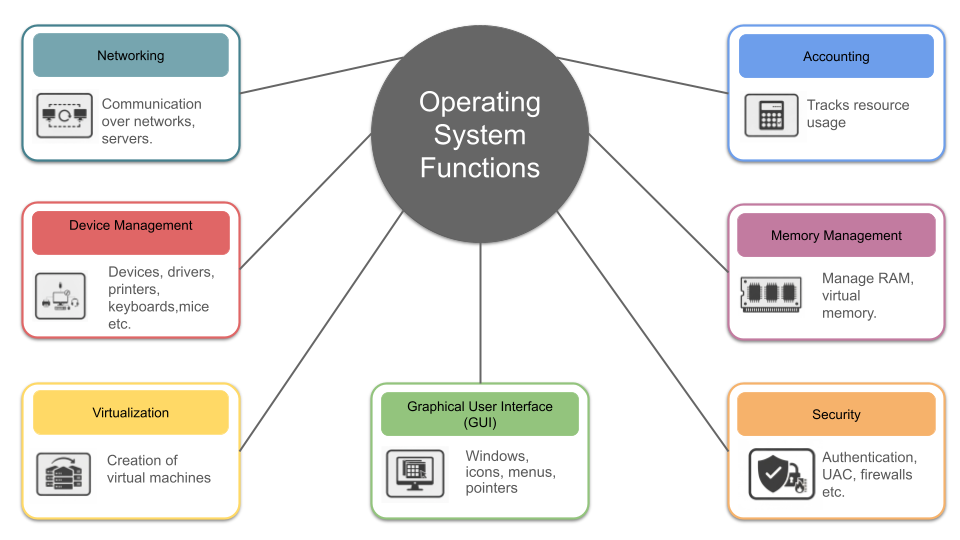
\includegraphics[width=0.7\linewidth]{os-functions.png}\\
    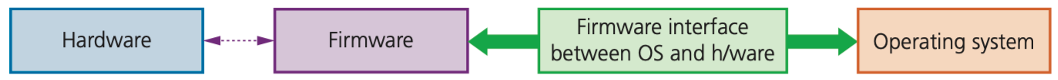
\includegraphics[width=0.8\linewidth]{Pasted 2026-10-20 at 14.06.09.png}
\end{center}
\paragraph{Approaches for scheduling}
An operating system needs scheduling methods to efficiently manage the execution of multiple processes, ensuring optimal use of the CPU and other resources. Without effective scheduling, processes could experience significant delays or monopolize resources (domination of system resources by a single process, reducing available resources for other processes, thereby slowing system down / inefficiency). The scheduler decides the order in which processes are granted CPU access and for how long, balancing the need for quick response to interactive applications against the efficient processing of long background tasks, so that the whole system stays responsive.
\begin{itemize}
    \item \textbf{First Come First Served (FCFS)}: processes are executed in the order they arrive in the ready queue. A process is added to the end of the queue on arrival; the CPU scheduler takes the process at the front and runs it until it completes or moves to an I/O wait state.
    \begin{itemize}
        \item Advantages: simple and easy to implement; fair, since requests are served in the order they arrived.
        \item Disadvantages: the \textit{convoy effect} --- a short process can be stuck behind a long-running one, so waiting times increase and throughput falls; it is non-pre-emptive, so once a process has the CPU it cannot be interrupted, wasting CPU time while it waits for I/O.
    \end{itemize}
    \item \textbf{Round Robin (RR)}: a pre-emptive, time-sharing algorithm. Every process is given a fixed time slice called a \textit{time quantum}; when the quantum expires the CPU pre-empts the process, moves it to the back of the ready queue and starts the next one. The cycle repeats until all processes finish.
    \begin{itemize}
        \item Advantages: fair allocation of CPU time between processes; high responsiveness and improved system interactivity; prevents any single process from monopolizing the CPU.
        \item Disadvantages: the quantum length is critical --- too short and the system spends most of its time context switching, too long and it degenerates into FCFS; processes that complete within a single quantum still cost a full switch.
    \end{itemize}
    \begin{center}
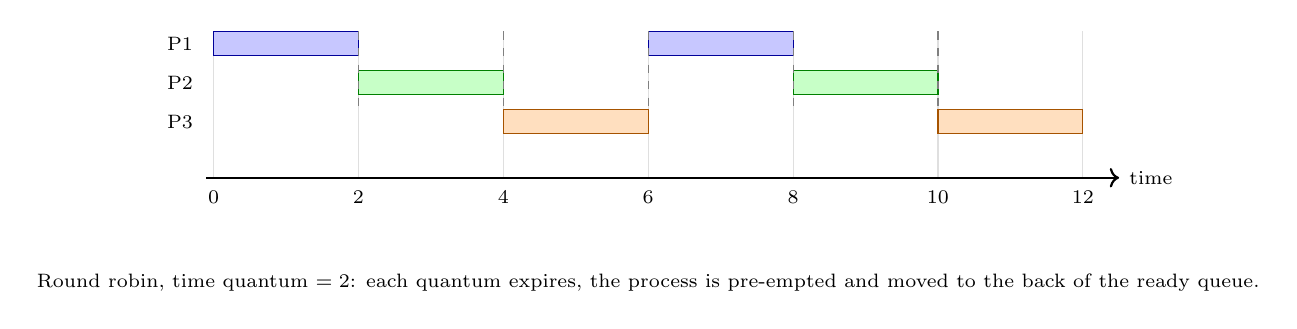
\begin{tikzpicture}[x=0.92cm,y=0.62cm,font=\small]
    \foreach \t in {0,2,4,6,8,10,12} {
        \draw[gray!25] (\t,0.35) -- (\t,3.35);
        \node[below,font=\scriptsize] at (\t,0.28) {\t};
    }
    \draw[->,thick] (-0.1,0.35) -- (12.5,0.35) node[right,font=\scriptsize]{time};
    \filldraw[fill=blue!22,draw=blue!60!black] (0,2.85) rectangle (2,3.35);
    \filldraw[fill=blue!22,draw=blue!60!black] (6,2.85) rectangle (8,3.35);
    \node[left,font=\scriptsize] at (-0.15,3.1) {P1};
    \filldraw[fill=green!22,draw=green!50!black] (2,2.05) rectangle (4,2.55);
    \filldraw[fill=green!22,draw=green!50!black] (8,2.05) rectangle (10,2.55);
    \node[left,font=\scriptsize] at (-0.15,2.3) {P2};
    \filldraw[fill=orange!25,draw=orange!65!black] (4,1.25) rectangle (6,1.75);
    \filldraw[fill=orange!25,draw=orange!65!black] (10,1.25) rectangle (12,1.75);
    \node[left,font=\scriptsize] at (-0.15,1.5) {P3};
    \draw[dashed,gray] (2,3.35) -- (2,1.75);
    \draw[dashed,gray] (4,3.35) -- (4,1.75);
    \draw[dashed,gray] (6,3.35) -- (6,1.75);
    \draw[dashed,gray] (8,3.35) -- (8,1.75);
    \draw[dashed,gray] (10,3.35) -- (10,1.75);
    \node[font=\scriptsize,below,yshift=-1.1cm] at (6,0.35) {Round robin, time quantum $=2$: each quantum expires, the process is pre-empted and moved to the back of the ready queue.};
\end{tikzpicture}
\end{center}

    \item \textbf{Priority scheduling}: each process is assigned a priority level and the CPU is allocated to the highest-priority ready process (equal priorities are broken by FCFS). Priority may be \textit{static} (fixed when the process is created) or \textit{dynamic} (changed over time, e.g. through ageing).
    \begin{itemize}
        \item Advantages: important and critical tasks are executed as soon as possible, improving responsiveness; flexible, because priorities can be adjusted dynamically as system needs change.
        \item Disadvantages: low-priority processes risk \textit{starvation} if high-priority processes continually take the CPU --- \textit{ageing} counteracts this by gradually increasing the priority of waiting processes; \textit{priority inversion} can arise when a lower-priority process holds a resource that a higher-priority process needs; more complex to implement and manage than FCFS.
    \end{itemize}
    \item \textbf{Multilevel queue scheduling}: the ready queue is partitioned into several separate queues, each with its own priority level and its own scheduling algorithm. Processes are permanently assigned to a queue by characteristics such as process type, priority or memory requirement; for example interactive processes sit in a high-priority queue scheduled with round robin, while batch processes sit in a lower-priority queue scheduled with FCFS. The scheduler always selects from the highest-priority queue, dropping to lower ones only when the higher queues are empty.
    \begin{itemize}
        \item Advantages: flexible handling of different types of processes; prioritizes critical and interactive processes, improving responsiveness; each queue can use the algorithm that best suits it.
        \item Disadvantages: complex implementation and management; starvation of lower-priority queues if the higher ones are frequently occupied; permanent queue assignment may be sub-optimal if a process's behaviour changes over time.
    \end{itemize}
    \item \textbf{Context switching}: when the CPU switches from one task to another, the state of the running process is saved and restored. It is what makes multitasking possible, but excessive switching reduces overall efficiency because the CPU spends its time saving and restoring tasks instead of doing useful work.
\end{itemize}
\textbf{Comparison chart}
\begin{center}
\renewcommand{\arraystretch}{1.5}
\begin{tabular}{|>{\raggedright\arraybackslash}p{3cm}|>{\raggedright\arraybackslash}p{5.5cm}|>{\raggedright\arraybackslash}p{4cm}|>{\raggedright\arraybackslash}p{4.5cm}|}
\hline
\textbf{Approach} & \textbf{How processor time is allocated} & \textbf{Main strength} & \textbf{Main limitation} \\ \hline
First-come first-served & In arrival order, each process runs to completion & Simple and predictable & Convoy effect: a long job delays all jobs behind it \\ \hline
Round robin & Fixed time slice each, then rotate to the back of the queue & Responsive; no process is starved & Frequent context switching adds overhead \\ \hline
Multilevel queue & Processes split into queues by type or priority, each queue with its own rule & Different work gets suitable treatment & Lower queues can starve; more complex to manage \\ \hline
Priority scheduling & Highest priority ready process runs first & Urgent and real-time work served first & Low priority processes can starve without ageing \\ \hline
\end{tabular}
\end{center}
\paragraph{Interrupt handling and polling}
Interrupt handling and polling are the two fundamental techniques for managing communication between the CPU and peripheral devices. Each has its own advantages and drawbacks, and which one is better depends entirely on the context of the system.
\begin{itemize}
    \item \textbf{Interrupt handling}: a peripheral device signals the CPU to request service. When an event occurs --- a keypress, data arriving on a network interface, a disk completing a read --- the device sends an \textit{interrupt signal}. The CPU pauses its current operations, saves its state and executes an \textit{interrupt service routine (ISR)} that addresses the event, before returning control to the main program. The CPU can therefore remain idle or perform other tasks until an event actually occurs.
    \begin{itemize}
        \item Advantages: highly efficient when events happen sporadically or unpredictably, because the CPU only deals with events when they occur and spends no cycles checking for them; preferred in real-time and interactive systems where an immediate response to events is crucial.
        \item Disadvantages: frequent interrupts introduce processing overhead through the context switching involved --- each ISR requires the CPU to save its current state and later restore it, which is time-consuming and resource-intensive if interrupts are too frequent; a high volume of interrupts also increases power consumption, which matters on battery-powered devices; if interrupts are too frequent, response times become unpredictable.
    \end{itemize}
    \item \textbf{Polling}: the CPU periodically checks each peripheral device to see whether it requires attention, at predetermined intervals.
    \begin{itemize}
        \item Advantages: straightforward and simple to implement; provides controlled latency with predictable response times, since checks occur at regular intervals; suitable for real-time applications whose events occur at regular, predictable intervals; adequate for simple embedded systems that are mostly idle.
        \item Disadvantages: significant CPU processing overhead, because the CPU repeatedly checks devices instead of doing useful work; resource-intensive and less power-efficient, since the CPU stays active continuously rather than idling; if the polling interval is too long, the detection of critical events is delayed.
    \end{itemize}
\end{itemize}
{\small
\setlength{\tabcolsep}{4pt}
\begin{longtable}{|>{\raggedright\arraybackslash}p{2.4cm}|>{\raggedright\arraybackslash}p{7.5cm}|>{\raggedright\arraybackslash}p{7.5cm}|}
\hline
\textbf{Aspect} & \textbf{Interrupt handling} & \textbf{Polling} \\
\hline
\endfirsthead
\hline
\textbf{Aspect} & \textbf{Interrupt handling} & \textbf{Polling} \\
\hline
\endhead
Event frequency & Efficient for infrequent, unpredictable events; the CPU responds only when an event occurs & Better for regular, predictable events; the CPU checks at set intervals regardless of whether anything happened \\
\hline
CPU overhead & Low for infrequent events, but rises with high-frequency interrupts due to context switching & Higher: constant device checking consumes cycles even when no event occurs \\
\hline
Power source & More power-efficient, especially on battery-powered devices, because the CPU idles until an event & Less power-efficient, because the CPU stays active continuously checking \\
\hline
Latency & Can respond quickly, but if interrupts are too frequent the response time becomes variable & Controlled, predictable latency, as checks occur at regular intervals \\
\hline
Security & Can react quickly to critical events, reducing the window for malicious activity & Less secure if the polling interval is too long, since critical events are detected late \\
\hline
\end{longtable}
}
\begin{center}
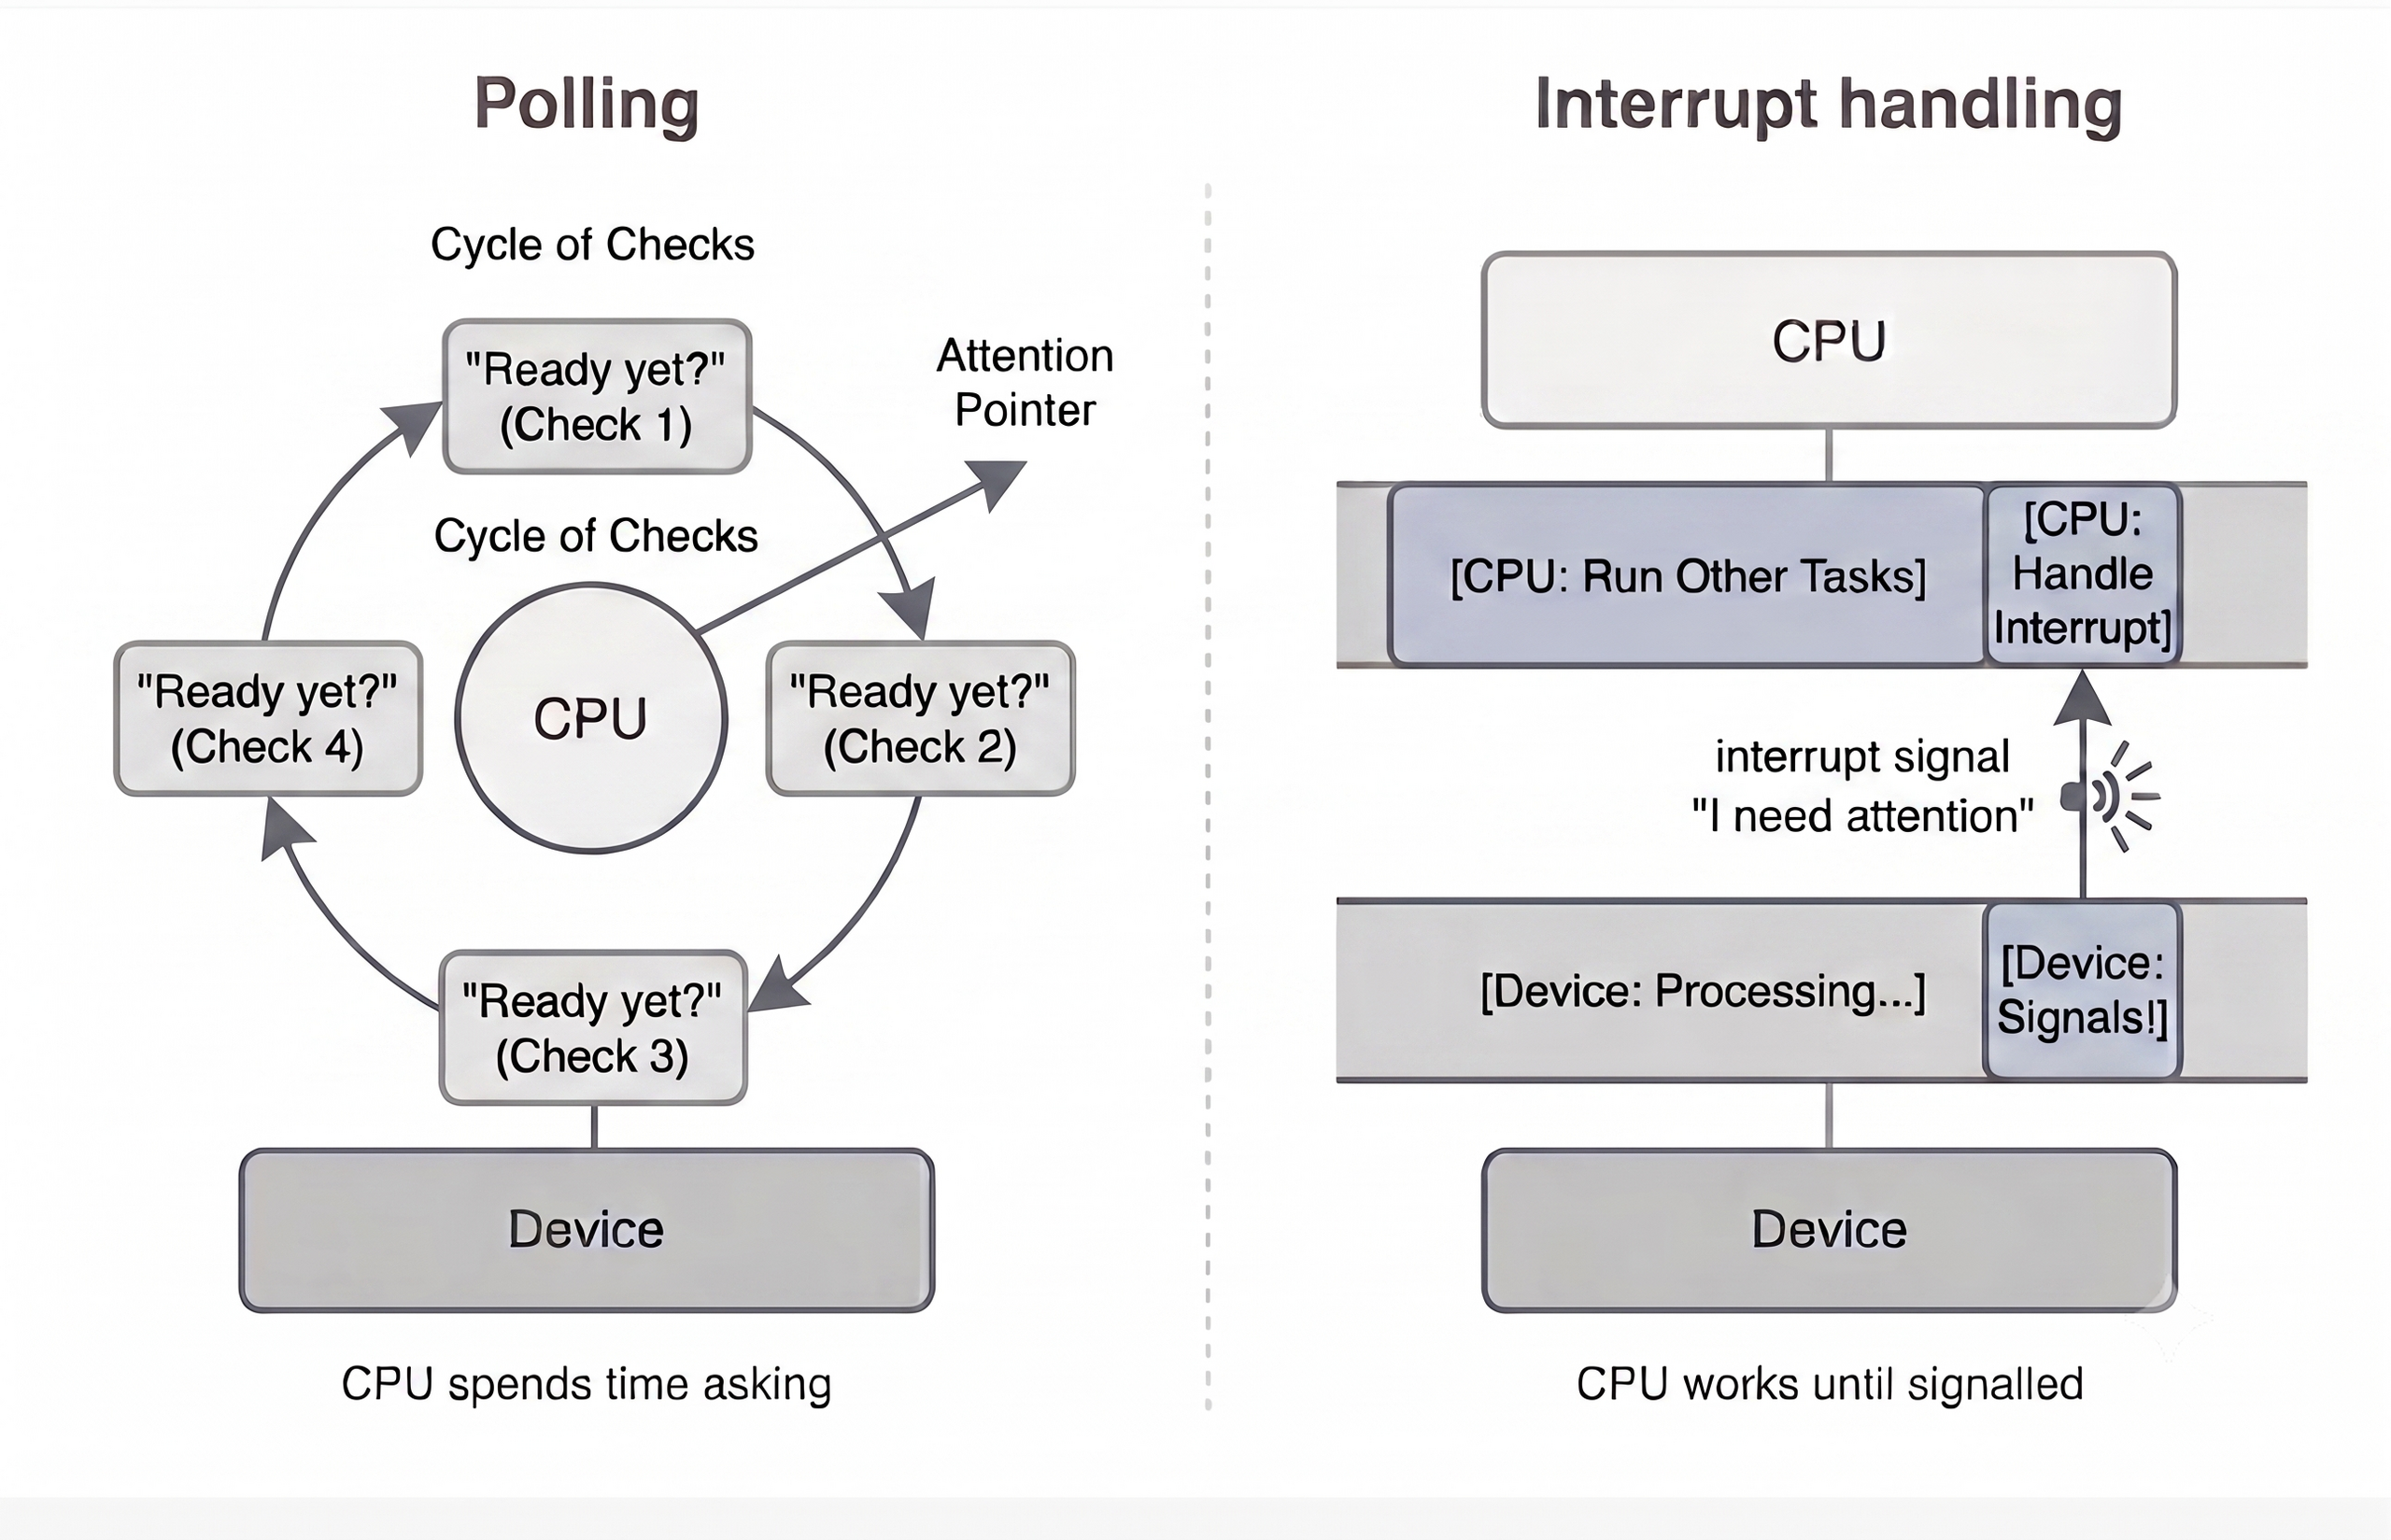
\includegraphics[width=0.7\linewidth]{polling_v_interrupt.png}
\end{center}
\textbf{Choosing between them (it is context, not one being better):}
\begin{itemize}
    \item \textit{Mouse and keyboard}: each keystroke generates an interrupt, so input is processed in real time with instant feedback; polling would force the CPU to check the devices continuously, wasting processing overhead and battery life, and could delay responses. In a simple kiosk or data-entry terminal that is mostly idle, polling at regular intervals is sufficient and simplifies the design.
    \item \textit{Network communication}: a network interface card (NIC) interrupts the CPU when data packets arrive, so data is received and passed to the application quickly, which is what keeps an audio/video conference at minimal latency; polling would mean constantly checking the NIC, increasing overhead and risking missed packets. Where traffic is minimal and predictable, such as a remote monitoring station sending small packets periodically, polling is more efficient.
    \item \textit{Disk input/output}: the disk interrupts the CPU when a read or write completes, so the CPU can execute other tasks while the operation finishes; polling would make the CPU waste cycles repeatedly checking for completion during lengthy disk operations. A data logger that writes at fixed intervals may find polling simpler.
    \item \textit{Embedded and real-time systems}: an automotive airbag sensor must interrupt the CPU immediately on impact, since a delayed response would be catastrophic; a climate-control system that samples temperature at regular intervals is a good candidate for polling, and an industrial robot performing repetitive fixed-interval tasks may prefer polling because it avoids the context-switching overhead and gives more predictable timing.
\end{itemize}
\paragraph{The role of the operating system in managing multitasking and resource allocation}
The OS plays a critical role in managing multitasking and resource allocation, ensuring that multiple processes can run concurrently and efficiently. \textit{Multitasking} allows a system to perform multiple tasks seemingly simultaneously by quickly switching between them, while \textit{resource allocation} ensures that each task receives the resources it needs (CPU time, memory, I/O devices) to execute properly.
\begin{itemize}
    \item \textbf{Task scheduling}: one of the primary responsibilities of the OS in a multitasking environment. The scheduler decides the order in which processes are executed, aiming to maximize CPU utilization and system responsiveness. It must balance the need for quick response times for interactive processes with the efficient processing of background tasks.
    \item \textbf{Resource contention}: occurs when multiple processes compete for the same resources, such as CPU time, memory or I/O devices. The OS must manage this contention to prevent conflicts and ensure fair and efficient resource usage. The key tool is \textit{mutual exclusion} --- preventing multiple processes from accessing a shared resource or \textit{critical section} simultaneously, so that only one process can use the resource at a time. This prevents data corruption and ensures consistency. Techniques for achieving mutual exclusion include \textit{semaphores}, \textit{locks} and \textit{monitors}.
    \begin{itemize}
        \item If contention is managed badly it leads to \textit{resource starvation}, where a process is constantly denied the resources it needs, or \textit{priority inversion}, where a lower-priority process holds a resource that a higher-priority process requires.
    \end{itemize}
    \item \textbf{Semaphores}: synchronization tools used to control access to shared resources in a concurrent system. A semaphore is an integer variable that can be incremented (\textit{signal}) or decremented (\textit{wait}) atomically.
    \begin{center}
    \begin{tabularx}{\linewidth}{|>{\raggedright\arraybackslash}p{3cm}|>{\raggedright\arraybackslash}X|>{\raggedright\arraybackslash}X|}
    \hline
    & \textbf{Binary semaphore (mutex)} & \textbf{Counting semaphore} \\
    \hline
    Possible values & Only 0 or 1, so it acts as a lock guaranteeing mutual exclusion & Any non-negative value \\
    \hline
    Purpose & Ensures that only one process enters the critical section at a time & Manages multiple instances of a resource \\
    \hline
    Typical use & Two processes writing to the same log file: the semaphore starts at 1 (available); Process A finds it at 1, sets it to 0 and writes; Process B finds 0 and is blocked until A finishes; A sets it back to 1, then B locks it, writes and restores it to 1 & Three database connections available: the semaphore starts at 3; each process that takes a connection decrements it by 1 (value reaches 0 when all three are in use); a fourth process must wait; when a process releases a connection it increments the semaphore by 1, freeing the waiting process \\
    \hline
    \end{tabularx}
    \end{center}
    \item \textbf{Locks}: tools that make sure only one process can use a shared resource at a time. If two programs want to write to the same file, the first must \textit{lock} the file before it can start writing; if the file is already locked by another program, the second has to wait until the lock is released. Types include \textit{binary locks} (also called mutexes), which allow only one process at a time, and \textit{readers-writer locks}, which let multiple processes read a resource but only one process write to it.
    \item \textbf{Monitors}: tools used in programming to manage access to shared resources safely. A monitor acts like a container holding shared variables and the code (methods) that works with them; when a process uses a monitor's method, the monitor is automatically locked so no other process can use it until the first one finishes. Monitors also have \textit{condition variables} that let processes wait for certain events to happen and notify others when those events occur, making it easier to co-ordinate tasks between processes safely.
    \item \textbf{Deadlock}: a problem in multitasking systems where processes get stuck because each one is waiting for a resource that another process holds, creating a cycle with no way to move forward.
    \begin{itemize}
        \item \textit{Prevention}: design the system so that deadlocks cannot happen.
        \item \textit{Avoidance}: use a strategy such as the \textbf{Banker's algorithm}, which only allocates resources if it can guarantee that all processes can eventually complete without entering an unsafe state.
        \item \textit{Detection}: regularly check for stuck processes, then take steps to fix the problem.
        \item \textit{Recovery}: stop one or more processes to break the cycle, or reallocate resources differently.
    \end{itemize}
    \item \textbf{Multitasking challenges}: the OS must also manage context-switching efficiently --- saving the state of the currently running process so that another process can be executed. Frequent context switches introduce overheads and reduce overall system performance. The OS must also ensure data consistency and integrity when multiple processes access shared data, by implementing robust synchronization mechanisms that prevent data corruption and stop processes interfering with each other.
\end{itemize}
\begin{center}
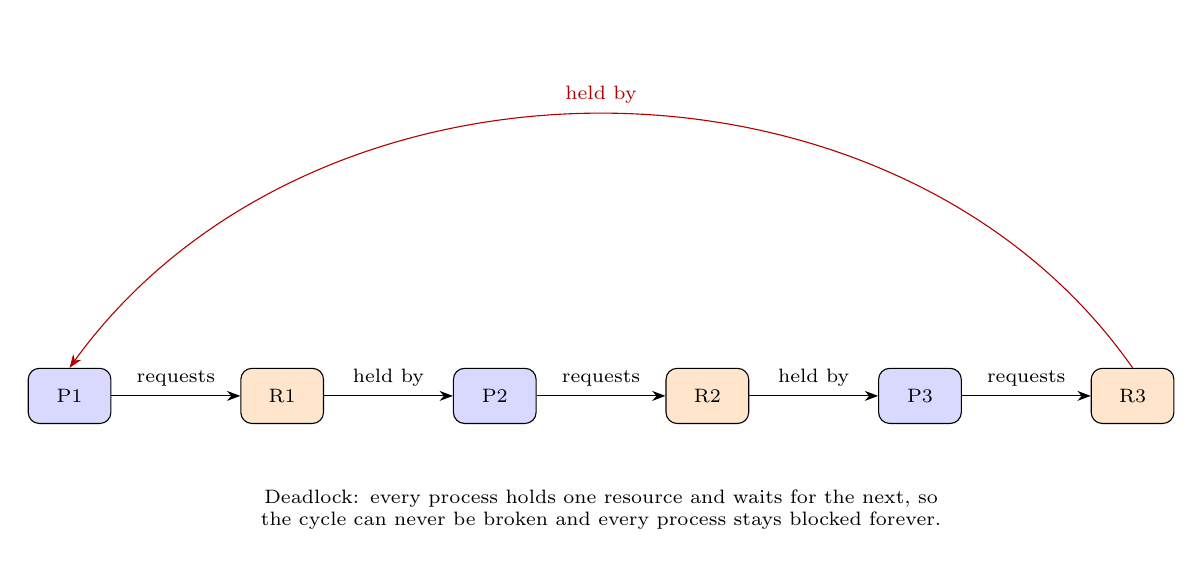
\begin{tikzpicture}[font=\scriptsize,>=Stealth]
    \node[draw,rounded corners,fill=blue!15,minimum width=1.05cm,minimum height=0.7cm] (P1) at (0,0) {P1};
    \node[draw,rounded corners,fill=orange!20,minimum width=1.05cm,minimum height=0.7cm] (R1) at (2.7,0) {R1};
    \node[draw,rounded corners,fill=blue!15,minimum width=1.05cm,minimum height=0.7cm] (P2) at (5.4,0) {P2};
    \node[draw,rounded corners,fill=orange!20,minimum width=1.05cm,minimum height=0.7cm] (R2) at (8.1,0) {R2};
    \node[draw,rounded corners,fill=blue!15,minimum width=1.05cm,minimum height=0.7cm] (P3) at (10.8,0) {P3};
    \node[draw,rounded corners,fill=orange!20,minimum width=1.05cm,minimum height=0.7cm] (R3) at (13.5,0) {R3};
    \draw[->] (P1) -- node[above,font=\scriptsize]{requests} (R1);
    \draw[->] (R1) -- node[above,font=\scriptsize]{held by} (P2);
    \draw[->] (P2) -- node[above,font=\scriptsize]{requests} (R2);
    \draw[->] (R2) -- node[above,font=\scriptsize]{held by} (P3);
    \draw[->] (P3) -- node[above,font=\scriptsize]{requests} (R3);
    \draw[->,red!70!black] (R3.north) to[out=125,in=55] node[above,font=\scriptsize,red!70!black]{held by} (P1.north);
    \node[font=\scriptsize,align=center,text width=14cm] at (6.75,-1.45) {Deadlock: every process holds one resource and waits for the next, so the cycle can never be broken and every process stays blocked forever.};
\end{tikzpicture}
\end{center}
\paragraph{The use of control system components}
Control systems are fundamental in automating and regulating processes across manufacturing, robotics and environmental control. At the core of any control system are components that work together to achieve desired outcomes by managing inputs, processing data and generating outputs, relying on a precise feedback mechanism to ensure the process remains stable and meets its set objectives.
\begin{itemize}
    \item \textbf{Input}: the initial signal or data received by the system, representing the desired condition or target that the system aims to achieve --- for example a set temperature in a heating system, or the desired speed in a motor-control application. It is typically generated by a user, another system or an environmental condition, and serves as the reference point for the system's operation.
    \item \textbf{Output}: the result produced by the control system after processing the input; it represents the actual state or action of the system, such as turning on a heater to reach a set temperature or adjusting the speed of a motor. The output is directly influenced by the input and the control process, and is typically the element that can be observed or measured to judge how effective the system is.
    \item \textbf{Feedback mechanism}: the critical component that determines how a control system operates and adjusts itself to maintain desired performance.
    \begin{itemize}
        \item \textit{Open-loop control}: there is no feedback from the output back to the input or the process. The system operates solely on the initial input, without any correction or adjustment based on the actual output. Simple, and used where the relationship between input and output is straightforward and predictable, such as basic timers or simple heating systems.
        \item \textit{Closed-loop control} (feedback control): the system continuously monitors the output and feeds that information back in to adjust the process. If the output deviates from the desired input, the system makes corrections in real time to bring the output back in line with the target. Essential where high accuracy and adaptability are required, such as temperature control in HVAC systems, where heating or cooling must be adjusted from actual temperature readings.
    \end{itemize}
\begin{center}
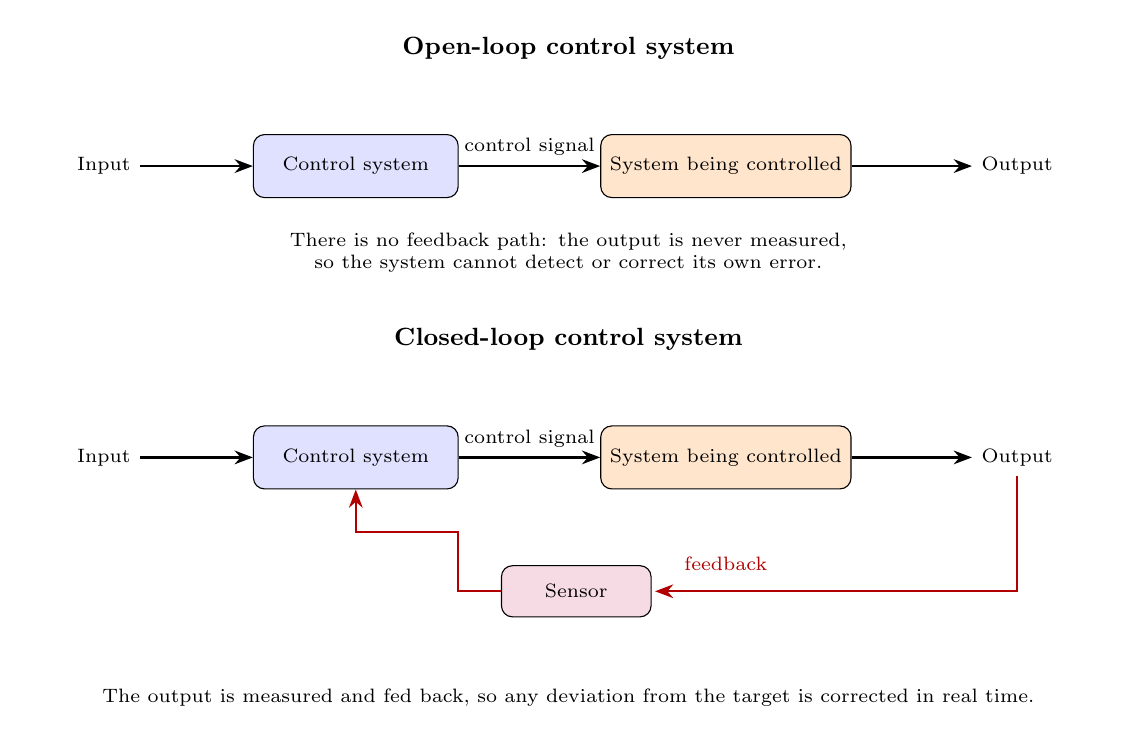
\begin{tikzpicture}[font=\scriptsize,>=Stealth]
% ---------- Open loop ----------
\node (oi) at (0,0) {Input};
\node[draw,rounded corners,fill=blue!12,minimum width=2.6cm,minimum height=0.8cm] (oc) at (3.2,0) {Control system};
\node[draw,rounded corners,fill=orange!20,minimum width=3.0cm,minimum height=0.8cm] (os) at (7.9,0) {System being controlled};
\node (oo) at (11.6,0) {Output};
\draw[->,thick] (oi) -- (oc);
\draw[->,thick] (oc) -- node[above,font=\scriptsize]{control signal} (os);
\draw[->,thick] (os) -- (oo);
\node[font=\small\bfseries] at (5.9,1.5) {Open-loop control system};
\node[font=\scriptsize,align=center,text width=13.5cm] at (5.9,-1.1) {There is no feedback path: the output is never measured, so the system cannot detect or correct its own error.};
% ---------- Closed loop ----------
\begin{scope}[yshift=-3.7cm]
\node (ci) at (0,0) {Input};
\node[draw,rounded corners,fill=blue!12,minimum width=2.6cm,minimum height=0.8cm] (cc) at (3.2,0) {Control system};
\node[draw,rounded corners,fill=orange!20,minimum width=3.0cm,minimum height=0.8cm] (cs) at (7.9,0) {System being controlled};
\node (co) at (11.6,0) {Output};
\draw[->,thick] (ci) -- (cc);
\draw[->,thick] (cc) -- node[above,font=\scriptsize]{control signal} (cs);
\draw[->,thick] (cs) -- (co);
\draw[->,thick,red!70!black] (co.south) -- (11.6,-1.7) -- (7.0,-1.7);
\node[draw,rounded corners,fill=purple!14,minimum width=1.9cm,minimum height=0.65cm] (sen) at (6.0,-1.7) {Sensor};
\draw[->,thick,red!70!black] (sen.west) -- (4.5,-1.7) -- (4.5,-0.95) -- (3.2,-0.95) -- (cc.south);
\node[font=\scriptsize,red!70!black] at (7.9,-1.35) {feedback};
\node[font=\small\bfseries] at (5.9,1.5) {Closed-loop control system};
\node[font=\scriptsize,align=center,text width=13.5cm] at (5.9,-3.05) {The output is measured and fed back, so any deviation from the target is corrected in real time.};
\end{scope}
\end{tikzpicture}
\end{center}
    \item \textbf{Controller}: the central component of a control system; it governs the operation by processing inputs and generating appropriate outputs. It is the ``brain'' of the system, implementing the control algorithm to make decisions based on the input data and feedback. It compares the input (desired value) with the feedback from the output (actual value) and determines the necessary actions to minimize the difference, or \textit{error}, between them, sending commands to actuators or other components. Controllers range from simple devices such as thermostats to complex microprocessors used in industrial automation.
    \item \textbf{Sensors}: devices that detect and measure physical quantities from the environment or the system itself, such as temperature, pressure, speed or light. The measurements are converted into electrical signals that the controller can interpret. Sensors are the ``eyes and ears'' of the control system; their accuracy and reliability directly affect performance, because they provide the critical feedback needed to adjust the system's operation --- e.g.\ a temperature sensor in a climate-control system constantly monitors the room temperature so the controller can adjust heating or cooling to maintain the setpoint.
    \item \textbf{Actuators}: the components that carry out the physical actions or adjustments in response to commands from the controller. They convert the controller's electrical signals into mechanical motion or other forms of energy, such as turning a valve, moving a robotic arm or adjusting a motor's speed. Actuators are the ``muscles'' of the control system, and their performance and precision are critical wherever exact control of movement or processes is required, such as manufacturing equipment and robotics.
    \item \textbf{Transducers}: devices that convert one form of energy into another, typically used to bridge the gap between sensors and actuators and the control system. Often a sensor or actuator cannot directly provide the type of signal the controller can process, or the signal needed to drive the actuator, so a transducer converts them into a compatible form --- e.g.\ a pressure sensor detecting mechanical pressure and converting it into an electrical signal the controller can interpret, or an actuator requiring a specific voltage or current supplied by a transducer. Transducers ensure that all parts of the control system can communicate effectively, enabling accurate and efficient operation.
    \item \textbf{Control algorithm}: the set of rules or mathematical procedures that the controller uses to determine the appropriate output from the input and feedback it receives; it is the logic driving decision-making within the controller. Complexity varies from simple \textit{proportional control}, where the output is adjusted in direct proportion to the error, to advanced methods such as \textit{Proportional-Integral-Derivative (PID)} control, which considers past, present and future errors to make precise adjustments. The choice depends on the system's requirements, such as desired accuracy, speed of response and stability.
\end{itemize}
\begin{center}
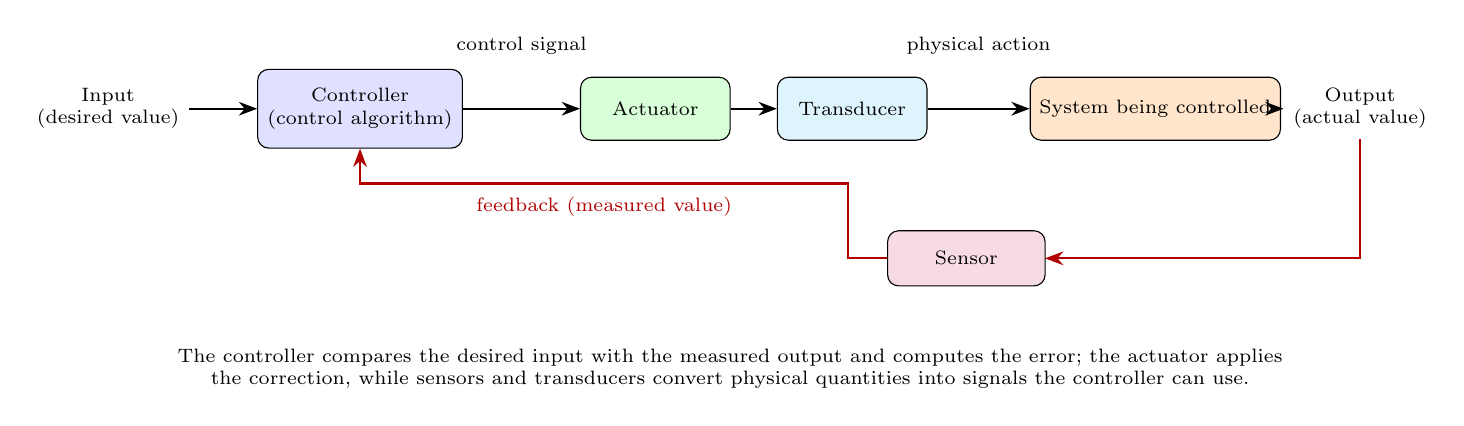
\begin{tikzpicture}[font=\scriptsize,>=Stealth]
\node[align=center] (bin) at (0,0) {Input\\(desired value)};
\node[draw,rounded corners,fill=blue!12,align=center,minimum width=2.6cm,minimum height=1.0cm] (bctrl) at (3.2,0) {Controller\\(control algorithm)};
\node[draw,rounded corners,fill=green!15,minimum width=1.9cm,minimum height=0.8cm] (bact) at (6.95,0) {Actuator};
\node[draw,rounded corners,fill=cyan!13,minimum width=1.9cm,minimum height=0.8cm] (btr) at (9.45,0) {Transducer};
\node[draw,rounded corners,fill=orange!20,minimum width=2.4cm,minimum height=0.8cm] (bsys) at (13.3,0) {System being controlled};
\node[align=center] (bout) at (15.9,0) {Output\\(actual value)};
\draw[->,thick] (bin) -- (bctrl);
\draw[->,thick] (bctrl) -- node[above=16pt,font=\scriptsize]{control signal} (bact);
\draw[->,thick] (bact) -- (btr);
\draw[->,thick] (btr) -- node[above=16pt,font=\scriptsize]{physical action} (bsys);
\draw[->,thick] (bsys) -- (bout);
\draw[->,thick,red!70!black] (bout.south) -- (15.9,-1.9) -- (11.9,-1.9);
\node[draw,rounded corners,fill=purple!14,minimum width=2.0cm,minimum height=0.7cm] (bsen) at (10.9,-1.9) {Sensor};
\draw[->,thick,red!70!black] (bsen.west) -- (9.4,-1.9) -- (9.4,-0.95) -- (3.2,-0.95) -- (bctrl.south);
\node[font=\scriptsize,red!70!black] at (6.3,-1.25) {feedback (measured value)};
\node[font=\scriptsize,align=center,text width=15cm] at (7.9,-3.3) {The controller compares the desired input with the measured output and computes the error; the actuator applies the correction, while sensors and transducers convert physical quantities into signals the controller can use.};
\end{tikzpicture}
\end{center}
\paragraph{The uses of control systems}
Every one of the following systems is a \textbf{closed-loop} system: the sensors continually send updated data back to the controller, and the controller adjusts its actions in real time in response.
{\small
\setlength{\tabcolsep}{4pt}
\begin{longtable}{|>{\raggedright\arraybackslash}p{2.6cm}|>{\raggedright\arraybackslash}p{3.3cm}|>{\raggedright\arraybackslash}p{7.4cm}|>{\raggedright\arraybackslash}p{3.0cm}|}
\hline
\textbf{System} & \textbf{Input (sensors)} & \textbf{Controller action} & \textbf{Output (actuators)} \\
\hline
\endfirsthead
\hline
\textbf{System} & \textbf{Input (sensors)} & \textbf{Controller action} & \textbf{Output (actuators)} \\
\hline
\endhead
Home thermostat & Temperature sensor continuously monitoring the room & Compares the current temperature with the desired setpoint and decides whether to activate heating or cooling & Heater, cooler / air conditioner \\
\hline
Automatic elevator & Position sensors, floor requests, door-status sensors & Processes the inputs to decide whether to move up or down, stop at a requested floor, or open and close the doors; adjusts the motor to slow down and halt precisely at the correct floor & Lift motor, door mechanism \\
\hline
Autonomous vehicle & Cameras, LiDAR, radar and GPS, gathering obstacles, road and traffic-signal data & Usually powered by advanced AI; runs control algorithms to make real-time decisions about speed, direction and braking & Steering, acceleration and braking systems \\
\hline
Washing machine & Water-level, load-size and cycle-progress sensors & Fills the drum with water, agitates the clothes and drains the water; stops filling once the required level is reached and adjusts the duration and intensity of the spin cycle to the detected load size & Motor, inlet valve, drain pump \\
\hline
Traffic signals & Sensors detecting vehicles, pedestrians and sometimes traffic conditions & Determines the timing and sequence of the lights (red, amber, green) for each direction; extends a green light for a congested lane or triggers a pedestrian crossing light & Signal lamps \\
\hline
Irrigation control & Soil-moisture, weather and sometimes time-of-day sensors & Decides when and how much water to deliver; activates the system when the soil is too dry and shuts off the supply once the desired moisture level is reached, conserving water and avoiding both under- and over-watering & Pumps and water valves \\
\hline
Home-security system & Door and window sensors, motion detectors, cameras & Assesses potential threats and determines the response, such as sounding an alarm, notifying the homeowner or contacting emergency services; locks doors or activates cameras to record an intrusion & Alarm, cameras, door locks, notification devices \\
\hline
Automatic doors & Infrared motion detectors or pressure mats detecting people or objects near the entrance & Decides when to open or close the doors; opens as soon as movement or pressure is detected and signals them to close once the person or object has passed and nothing is detected & Door motor \\
\hline
\end{longtable}
}
\textbf{Exam pointers:}
\begin{itemize}
    \item In every example the \textit{input} is a physical quantity measured by a sensor, the \textit{output} is a physical action performed by an actuator, and the \textit{feedback} is the measured result being returned to the controller.
    \item The key difference between open-loop and closed-loop shows up clearly here: a closed-loop system (thermostat, elevator, washing machine) can correct itself when the actual value drifts from the target, whereas a purely open-loop system (e.g.\ a simple timer) cannot.
    \item Autonomous vehicles and elevators are the best examples to use when explaining why \textit{transducers} matter: sensors such as LiDAR and radar produce signals that the controller cannot use directly, and actuators such as steering and braking need precisely shaped electrical signals, so transducers convert between the physical world and the electronic signals.
\end{itemize}
\subsubsection{Translation}
\paragraph{Translation processes of interpreters and compilers}
Interpreters and compilers both transform high-level code into machine-readable instructions, yet they do so through different methods, each with unique implications for performance, error handling and development efficiency.
\begin{itemize}
    \item \textbf{Interpreters}: translate high-level programming code into machine code \emph{line-by-line or statement-by-statement}, executing each line as it is translated. Unlike compilers, they do not generate an intermediate machine-code file; instead they directly execute the source code on the fly, reading the code, translating it and running it immediately, and repeating this for each line or block until the whole program has been executed.
    \begin{itemize}
        \item \textit{Mechanics}: an interpreter can start executing a program without processing the entire codebase upfront, which allows for immediate feedback --- particularly useful during development and debugging. The cost is slower overall performance, since the code must be repeatedly translated and executed on every run.
        \item \textit{Use cases}: quick testing and debugging are essential; languages such as Python, JavaScript and Ruby are often interpreted, making them popular for web development, scripting and rapid application development. Interpreters are also ideal for educational purposes, enabling beginners to see results in real time, and are favoured where portability matters, since the same source code runs on any platform that has the appropriate interpreter.
    \end{itemize}
    \item \textbf{Compilers}: translate the \emph{entire} high-level source code into machine code in a single, comprehensive process \emph{before} the program is executed. This involves several stages: \textbf{lexical analysis} (breaking the source into tokens), \textbf{syntax analysis} (checking the tokens form valid code), \textbf{semantic analysis} (checking the code actually makes sense), \textbf{optimization} and \textbf{code generation}. The final output is a standalone executable file, typically in machine code or an intermediate form such as bytecode, which can be run directly on the target machine.
    \begin{itemize}
        \item \textit{Mechanics}: once compiled, the machine code needs no further translation, so the program executes much faster than interpreted code. However the initial compilation can be time-consuming, especially for large and complex programs, and because the whole code must be compiled before execution, any source errors have to be addressed first, which slows the development cycle.
        \item \textit{Use cases}: performance-critical software, where languages including C, C++ and Java (which compiles to bytecode for the JVM) are suited to system software, high-performance computing and real-time systems such as video games. Compiled code is also advantageous where security and resource control matter, since pre-generated, optimized machine code is harder to reverse-engineer and is less dependent on external environments. Finally, compilers are often chosen when software must be deployed across different hardware specifications, since compilation can be tailored to optimize the executable for specific architectures.
    \end{itemize}
    \item \textbf{Bytecode interpreters}: first translate the high-level source code into an intermediate form known as \textbf{bytecode}. This bytecode is not executed by the machine's hardware directly, but by a \textbf{virtual machine (VM)} or an interpreter that understands the bytecode's instructions. Bytecode is a compact, platform-independent representation of the program, so it can run on any system with the appropriate VM.
    \begin{itemize}
        \item \textit{Use cases}: Java is the prime example --- code is compiled into bytecode that runs on the Java Virtual Machine (JVM), so the same application runs on any platform with a JVM, making it ideal for enterprise applications, web services and mobile apps. Python uses a similar approach, compiling source to bytecode (the \texttt{.pyc} file) which is then executed by the Python interpreter, so bytecode interpreters are also valuable in educational settings, web development and scripting, where flexibility and ease of deployment matter more than raw performance.
    \end{itemize}
    \item \textbf{Just-in-time (JIT) compilation}: a dynamic approach that combines elements of both interpretation and compilation. Initially the source code is compiled into bytecode, which is then interpreted by a virtual machine. As the program runs, the JIT compiler identifies frequently executed sections of the bytecode --- the \textit{hot spots} --- and compiles them into machine code on the fly. This machine code is then cached, so the next time the same code is executed the system uses the compiled version instead of interpreting it again.
    \begin{itemize}
        \item \textit{Use cases}: beneficial where performance is critical but the application must also stay portable and dynamically optimized. Both the JVM and the .NET runtime use JIT compilation, and it is especially valuable in long-running applications such as servers, where the overhead of JIT compilation is outweighed by the gains on subsequent runs of the same code paths. Web browsers also use it to optimize frequently executed JavaScript and improve page load times.
    \end{itemize}
\end{itemize}
\begin{center}
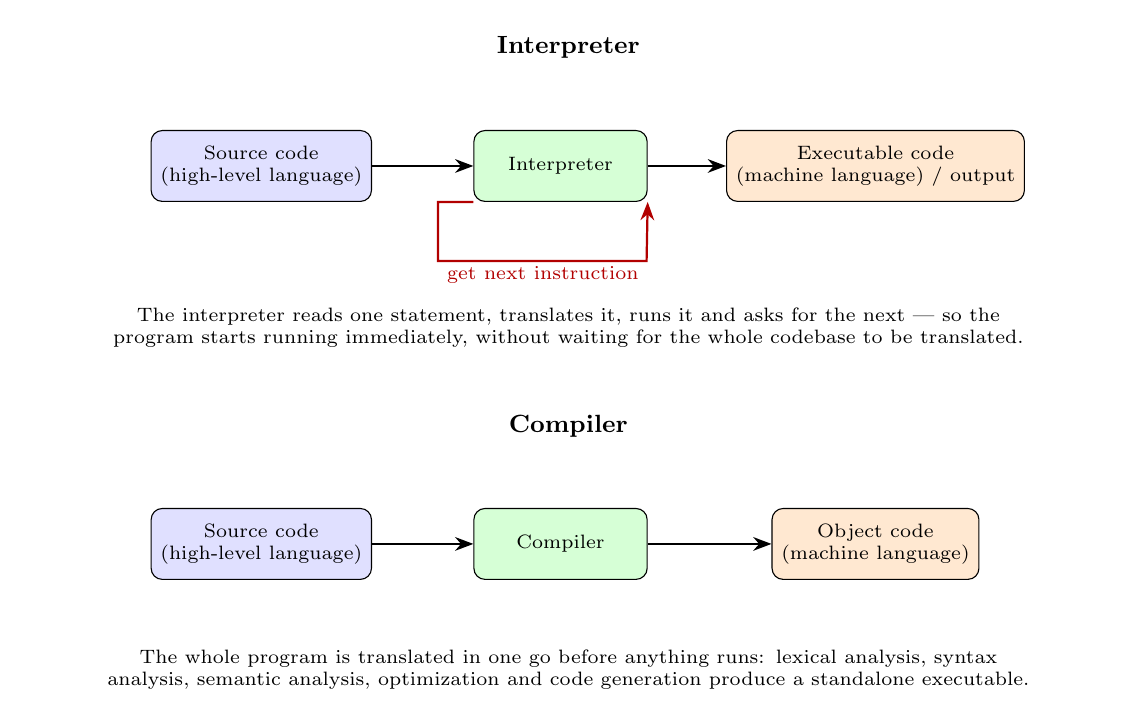
\begin{tikzpicture}[font=\scriptsize,>=Stealth]
% ---------- Interpreter ----------
\node[draw,rounded corners,fill=blue!12,align=center,minimum width=2.4cm,minimum height=0.9cm] (src1) at (0,0) {Source code\\(high-level language)};
\node[draw,rounded corners,fill=green!16,align=center,minimum width=2.2cm,minimum height=0.9cm] (int1) at (3.8,0) {Interpreter};
\node[draw,rounded corners,fill=orange!18,align=center,minimum width=2.6cm,minimum height=0.9cm] (out1) at (7.8,0) {Executable code\\(machine language) / output};
\draw[->,thick] (src1) -- (int1);
\draw[->,thick] (int1) -- (out1);
\draw[->,thick,red!70!black] (int1.south west) -- ++(-0.45,0) -- ++(0,-0.75) -- ++(2.65,0) -- (int1.south east);
\node[font=\scriptsize,red!70!black] at (3.575,-1.38) {get next instruction};
\node[font=\small\bfseries] at (3.9,1.5) {Interpreter};
\node[font=\scriptsize,align=center,text width=13.5cm] at (3.9,-2.05) {The interpreter reads one statement, translates it, runs it and asks for the next --- so the program starts running immediately, without waiting for the whole codebase to be translated.};
% ---------- Compiler ----------
\begin{scope}[yshift=-4.8cm]
\node[draw,rounded corners,fill=blue!12,align=center,minimum width=2.4cm,minimum height=0.9cm] (src2) at (0,0) {Source code\\(high-level language)};
\node[draw,rounded corners,fill=green!16,align=center,minimum width=2.2cm,minimum height=0.9cm] (cmp2) at (3.8,0) {Compiler};
\node[draw,rounded corners,fill=orange!18,align=center,minimum width=2.6cm,minimum height=0.9cm] (obj2) at (7.8,0) {Object code\\(machine language)};
\draw[->,thick] (src2) -- (cmp2);
\draw[->,thick] (cmp2) -- (obj2);
\node[font=\small\bfseries] at (3.9,1.5) {Compiler};
\node[font=\scriptsize,align=center,text width=13.5cm] at (3.9,-1.6) {The whole program is translated in one go before anything runs: lexical analysis, syntax analysis, semantic analysis, optimization and code generation produce a standalone executable.};
\end{scope}
\end{tikzpicture}
\end{center}
\begin{center}
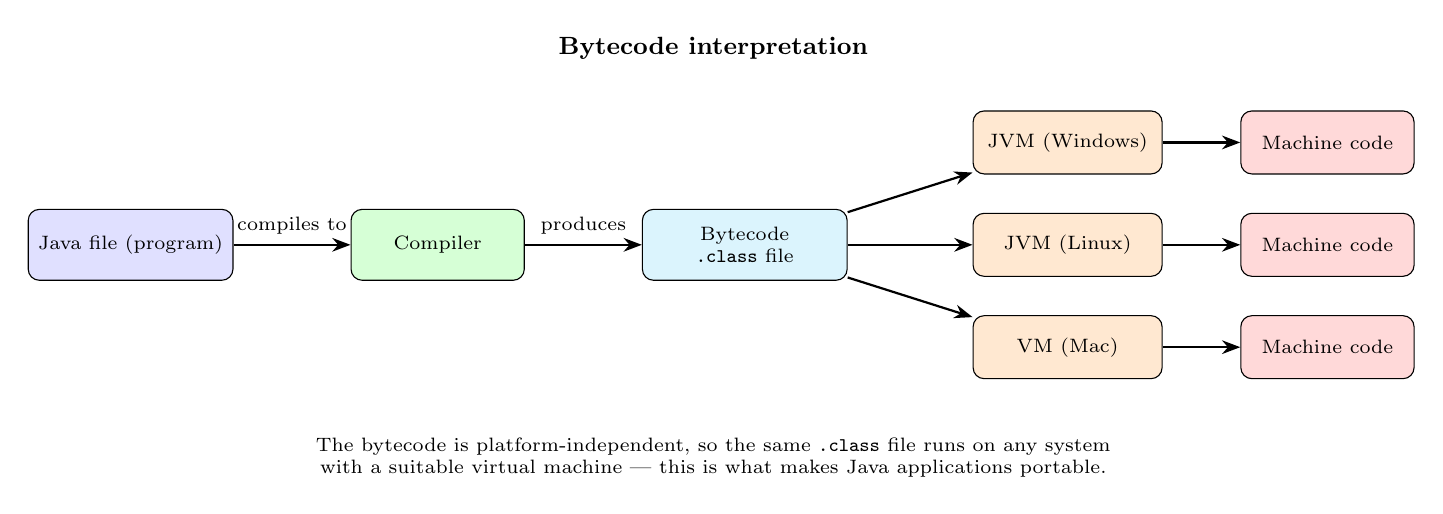
\begin{tikzpicture}[font=\scriptsize,>=Stealth]
\node[draw,rounded corners,fill=blue!12,align=center,minimum width=2.6cm,minimum height=0.9cm] (jf) at (0,0) {Java file (program)};
\node[draw,rounded corners,fill=green!16,minimum width=2.2cm,minimum height=0.9cm] (jc) at (3.9,0) {Compiler};
\node[draw,rounded corners,fill=cyan!14,align=center,minimum width=2.6cm,minimum height=0.9cm] (bc) at (7.8,0) {Bytecode\\\texttt{.class} file};
\draw[->,thick] (jf) -- node[above,font=\scriptsize]{compiles to} (jc);
\draw[->,thick] (jc) -- node[above,font=\scriptsize]{produces} (bc);
\node[draw,rounded corners,fill=orange!18,align=center,minimum width=2.4cm,minimum height=0.8cm] (jvmw) at (11.9,1.3) {JVM (Windows)};
\node[draw,rounded corners,fill=orange!18,align=center,minimum width=2.4cm,minimum height=0.8cm] (jvml) at (11.9,0) {JVM (Linux)};
\node[draw,rounded corners,fill=orange!18,align=center,minimum width=2.4cm,minimum height=0.8cm] (jvmm) at (11.9,-1.3) {VM (Mac)};
\node[draw,rounded corners,fill=red!15,align=center,minimum width=2.2cm,minimum height=0.8cm] (mc1) at (15.2,1.3) {Machine code};
\node[draw,rounded corners,fill=red!15,align=center,minimum width=2.2cm,minimum height=0.8cm] (mc2) at (15.2,0) {Machine code};
\node[draw,rounded corners,fill=red!15,align=center,minimum width=2.2cm,minimum height=0.8cm] (mc3) at (15.2,-1.3) {Machine code};
\draw[->,thick] (bc) -- (jvmw);
\draw[->,thick] (bc) -- (jvml);
\draw[->,thick] (bc) -- (jvmm);
\draw[->,thick] (jvmw) -- (mc1);
\draw[->,thick] (jvml) -- (mc2);
\draw[->,thick] (jvmm) -- (mc3);
\node[font=\small\bfseries] at (7.4,2.5) {Bytecode interpretation};
\node[font=\scriptsize,align=center,text width=14cm] at (7.4,-2.7) {The bytecode is platform-independent, so the same \texttt{.class} file runs on any system with a suitable virtual machine --- this is what makes Java applications portable.};
\end{tikzpicture}
\end{center}
\begin{center}
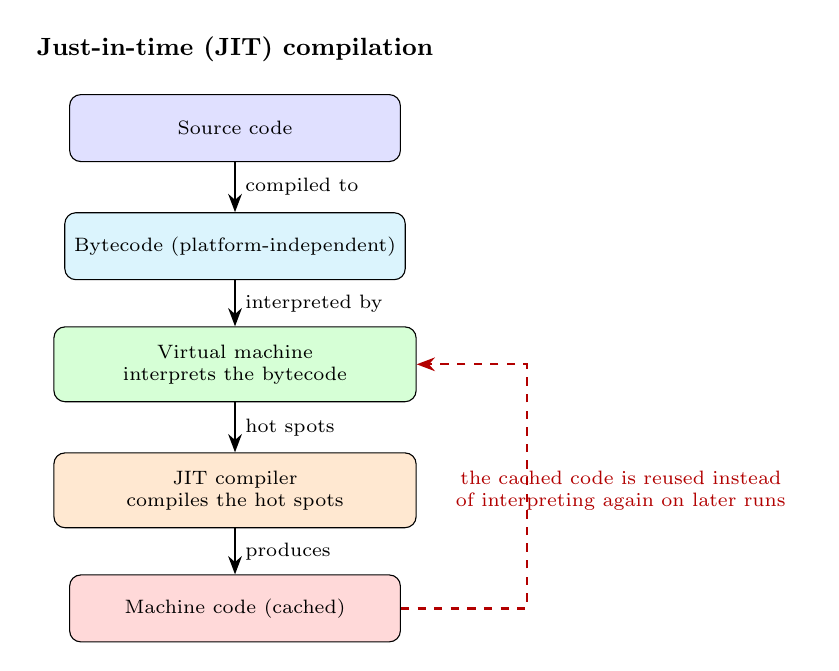
\begin{tikzpicture}[font=\scriptsize,>=Stealth]
\node[draw,rounded corners,fill=blue!12,minimum width=4.2cm,minimum height=0.85cm] (jsrc) at (0,0) {Source code};
\node[draw,rounded corners,fill=cyan!14,minimum width=4.2cm,minimum height=0.85cm] (jbc) at (0,-1.5) {Bytecode (platform-independent)};
\node[draw,rounded corners,fill=green!16,align=center,minimum width=4.6cm,minimum height=0.95cm] (jvm) at (0,-3.0) {Virtual machine\\interprets the bytecode};
\node[draw,rounded corners,fill=orange!18,align=center,minimum width=4.6cm,minimum height=0.95cm] (jjit) at (0,-4.6) {JIT compiler\\compiles the hot spots};
\node[draw,rounded corners,fill=red!15,minimum width=4.2cm,minimum height=0.85cm] (jmc) at (0,-6.1) {Machine code (cached)};
\draw[->,thick] (jsrc) -- node[right,font=\scriptsize]{compiled to} (jbc);
\draw[->,thick] (jbc) -- node[right,font=\scriptsize]{interpreted by} (jvm);
\draw[->,thick] (jvm) -- node[right,font=\scriptsize]{hot spots} (jjit);
\draw[->,thick] (jjit) -- node[right,font=\scriptsize]{produces} (jmc);
\draw[->,thick,dashed,red!70!black] (jmc.east) -- ++(1.6,0) -- ++(0,3.1) -- (jvm.east);
\node[font=\scriptsize,red!70!black,align=center,text width=4.6cm] at (4.9,-4.6) {the cached code is reused instead of interpreting again on later runs};
\node[font=\small\bfseries] at (0,1.0) {Just-in-time (JIT) compilation};
\end{tikzpicture}
\end{center}
\begin{center}
\textbf{\textit{Top tip:}}\quad An interpreter is like someone who translates each sentence of a book for you as you read, giving you immediate understanding, but requiring them to translate each line again every time you revisit it. A compiler is like a translator who first converts the entire book into your native language, letting you read it smoothly without any further translation --- but you have to wait until the whole book is translated before you can start reading.
\end{center}
\paragraph{Evaluating the translation processes}
\begin{itemize}
    \item \textbf{Error detection}: compilers offer the most robust detection, because they analyse the entire source code before producing an executable, so all syntax and some semantic errors are caught and must be resolved before the program can run --- giving fewer runtime errors and a more stable final product. Interpreters detect errors at run time, as they execute code line by line, which lets developers quickly identify and correct errors during development; the downside is that errors are only discovered when the offending code actually executes, so a runtime error can disrupt execution unexpectedly. Bytecode interpreters provide a middle ground: some errors are caught before execution, but others still appear at run time, reducing the frequency of runtime errors without offering the exhaustive checking of full compilation. JIT combines runtime error detection with dynamic optimization.
    \item \textbf{Translation time}: compilers require a considerable amount of time initially to convert the entire source code, but the payoff is that the compiled program runs significantly faster once translation is complete. Interpreters execute code directly by translating it line by line, so the program runs almost immediately, which is advantageous for quick testing and iterating; however, larger codebases experience slower overall performance. Bytecode interpreters balance the two --- compiling to bytecode is quicker than compiling to machine code, and bytecode then executes more efficiently than direct interpretation of source. JIT goes a step further by converting bytecode into machine code dynamically as the program runs: some runtime overhead, but it reduces initial translation time while improving execution speed as the program continues, especially for frequently executed code paths.
    \item \textbf{Portability}: a significant advantage of interpreters and bytecode interpreters. Since interpreters execute source code directly, the same code runs on any platform with the appropriate interpreter, making them ideal for cross-platform applications. Bytecode interpreters extend this by compiling source into platform-independent bytecode that runs on any system with the appropriate VM (for example Java's JVM), which is particularly valuable where applications must operate across diverse platforms without modification. Compilers, however, produce machine code tailored to specific hardware architectures, resulting in highly efficient but far less portable executables --- each target platform may require separate compilation. JIT preserves the portability of bytecode while enhancing performance, optimizing for the specific hardware at runtime.
    \item \textbf{Applicability}: compilers are best suited to applications where performance is critical, such as system software, high-performance computing and real-time systems, since the upfront compilation time is justified by the high execution speed of the resulting code. Interpreters are ideal for scenarios where rapid development, testing and iteration are essential --- scripting, web development and educational environments --- where flexibility and quick feedback matter more than raw performance. Bytecode interpreters are commonly used in enterprise applications, web services and mobile apps where cross-platform compatibility is crucial, offering a flexible balance of portability and efficient execution. JIT compilation is particularly valuable in long-running applications and complex systems where performance needs to improve over time --- server environments, dynamic web applications, and platforms such as Java and .NET.
\end{itemize}
\textbf{Comparison Chart}
\begin{center}
% \renewcommand{\arraystretch}{1.5} % Adds vertical padding to rows
\begin{tabular}{| p{2.8cm} | p{3.5cm} | p{3.5cm} | p{3.5cm} | p{3.5cm} |}
\hline
\bfseries  & \bfseries Interpreter & \bfseries Compiler & \bfseries JIT compiler & \bfseries Bytecode interpreter \\
\hline
\bfseries Error detection & At run time, as each statement is reached & At compile time, before execution & At run time; verification can catch some errors first & At run time; bytecode verification catches some errors first \\
\hline
\bfseries Translation time & Negligible; starts at once & Slow; whole program translated upfront & Fast start, then compiles hot code during the run & Faster than full compilation; bytecode is an intermediate step \\
\hline
\bfseries Execution speed & Slower; translation continues throughout & Fast; optimised native code & Near-compiled on hot paths & Faster than direct interpretation, below native \\
\hline
\bfseries Portability & High; runs anywhere the interpreter exists & Low; native code is platform-specific & Moderate; tuned to the host at run time & High; same bytecode runs on any compatible VM \\
\hline
\bfseries Applicability & Scripting, prototyping, dynamic languages & Performance-critical and systems software & Balance of portability and speed & Portable apps with moderate performance needs \\
\hline
\end{tabular}
\end{center}
\paragraph{Example scenarios}
\begin{center}
\begin{tabular}{| p{3.4cm} | p{3.6cm} | p{9.4cm} |}
\hline
\bfseries Scenario & \bfseries Best translation method & \bfseries Explanation \\
\hline
Rapid development and testing & Interpreters & Immediate execution allows quick iterations, debugging and real-time feedback; ideal for scripting languages such as Python or JavaScript \\
\hline
Performance-critical applications & Compilers & The whole codebase is optimized into machine code before execution, giving highly efficient, fast-running applications; suitable for system software, gaming and real-time systems in C or C++ \\
\hline
Cross-platform development & Bytecode interpreters and JIT compilation & Bytecode gives platform independence (the same code runs on any platform with the right VM), while JIT enhances performance by optimizing frequently executed code at runtime; ideal for enterprise software, mobile apps and web services \\
\hline
\end{tabular}
\end{center}
\subsection{Networks}
\subsubsection{Network fundamentals}
\subsubsection{Network architecture}
\subsubsection{Data transmission}
\subsubsection{Network security}
\subsection{Databases}
\subsubsection{Database fundamentals}
\subsubsection{Database design}
\subsubsection{Database programming}
\subsubsection{Alternative databases and data warehouses}
\subsection{Machine learning}
\subsubsection{Machine learning fundamentals}
\subsubsection{Data preprocessing}
\subsubsection{Machine learning approaches}
\subsubsection{Ethical considerations}

\newpage
\section{Computational Thinking and Problem Solving}
\subsection{Computational thinking}
\subsubsection{Approaches to computational thinking}
\paragraph{Problem specification}
\paragraph{Fundamental concepts of computational thinking}
\begin{itemize}
    \item Abstraction
    \begin{itemize}
        \item Definition: the process of extracting essential information, while disregarding irrelevant data, to propose or outline a feasible solution to a given problem.
        \item Why it is important: Hide complexity from the user by abstracting data entities and hiding underlying implementation of a process.
        \item By using abstraction: the time required to create a piece of software is reduced; the program becomes smaller in size, so it requires less space in memory and the download times are reduced; customer satisfaction increases, as their requirements are met without extra features. 
    \end{itemize}
\end{itemize}

\subsection{Programming}
\subsubsection{Programming fundamentals}
\subsubsection{Programming constructs}
\subsubsection{Data structures}
\subsubsection{Programming algorithms}
\subsubsection{File processing}
\subsection{Object-oriented programming (OOP)}
\subsubsection{Fundamentals of OOP for a single class}
\subsubsection{Fundamentals of OOP for multiple classes}
\subsection{Abstract data types (ADTs)}
\subsubsection{Fundamentals of abstract data types}
\newpage
\section{Appendices}
\subsubsection{My favourite operating system: Arch Linux (+ Hyprland)}
\paragraph{What it is}
Arch Linux is a lightweight, rolling-release distribution built around the principle of user-centricity: you start from a minimal base and build up exactly the system you want, installing only the packages you actually need. On top of it I run Hyprland, a dynamic tiling Wayland compositor, which handles all the window management and visual effects. Together they are not a finished product you install, but a system you assemble and shape yourself.
\paragraph{Why it is my favourite}
\begin{itemize}
    \item Customizability: nothing is assumed for me. Every package, service, kernel module and keybind is a deliberate choice, so the OS fits my workflow instead of the other way around. Hyprland is configured entirely through a plain-text file, so layouts, animations and rules can be tuned down to the pixel.
    \item Responsiveness and performance: the system ships with no bundled bloatware or background services, so boot times are short and idle resource usage is very low. On the same hardware, a minimal Arch + Hyprland setup feels noticeably snappier than a stock desktop environment.
    \item Rolling release: packages are updated continuously rather than frozen until the next major version, so I always have current kernels, drivers and toolchains without a disruptive reinstall.
    \item The AUR and community: the Arch User Repository gives access to an enormous range of community-maintained packages, and the Arch Wiki is arguably the best-documented Linux resource available, which makes troubleshooting a learning exercise rather than a dead end.
    \item Keyboard-driven workflow: as a tiling compositor, Hyprland automatically arranges windows with no manual dragging, which keeps my hands on the keyboard, reduces context switching and makes multitasking far faster.
    \item Learning and control: because I built the system, I understand how each layer fits together. Using Arch teaches real operating-system concepts — package management, the boot process, display servers, resource allocation — which connects directly back to the OS material in Section A.
\end{itemize}
A rolling-release, build-it-yourself system does come with trade-offs: upgrades occasionally break things and demand manual intervention, and there is no vendor support to fall back on. For me that trade-off is worth it — the control and understanding I gain outweigh the convenience I give up.

\end{document}
